%Version 3.1 December 2024
%% Multi-paradigm benchmarking for integrated soil quality assessment
%% Manuscript EN-US (submission version)
%%
%%%%%%%%%%%%%%%%%%%%%%%%%%%%%%%%%%%%%%%%%%%%%%%%%%%%%%%%%%%%%%%%%%%%%%

\documentclass[pdflatex,sn-basic]{sn-jnl}% Basic Springer Nature Reference Style

%%%% Standard Packages
\usepackage{graphicx}%
\usepackage{multirow}%
\usepackage{amsmath,amssymb,amsfonts}%
\usepackage{amsthm}%
\usepackage{mathrsfs}%
\usepackage[title]{appendix}%
\usepackage{xcolor}%
\usepackage{textcomp}%
\usepackage{manyfoot}%
\usepackage{booktabs}%
\usepackage{algorithm}%
\usepackage{algorithmicx}%
\usepackage{algpseudocode}%
\usepackage{listings}%
\usepackage{tikz}%
\usetikzlibrary{shapes.geometric, arrows.meta, positioning, calc}%
\usepackage{subcaption}%
\raggedbottom

\begin{document}

\title[Analytical uncertainty and stochastic risk]{Analytical uncertainty of the statistical paradigm as a vector of stochastic risk in soil quality assessment under long-term conservation management}

%%=============================================================%%
%% Authors
%%=============================================================%%

\author[1]{\fnm{Alceu} \sur{Pedrotti}}\email{alceupedrotti@gmail.com}

\author*[2]{\fnm{Luiz Diego Vidal} \sur{Santos}}\email{ldvsantos@uefs.br}

\author[1]{\fnm{Jusimara de Andrade} \sur{Santos}}\email{jusimara.ufs@gmail.com}

\author[4]{\fnm{Jaelson Souza} \sur{Ara\'{u}jo}}\email{jaelsonagro1207@gmail.com}

\author[4]{\fnm{Emersson Guedes da} \sur{Silva}}\email{academicoguedes@gmail.com}

\author[3]{\fnm{Renisson Neponuceno de} \sur{Ara\'{u}jo Filho}}\email{renisson.neponuceno@ufrpe.br}

\author[1]{\fnm{Brisa Marina da Silva} \sur{Andrade}}\email{brisamarina.andrade@gmail.com}

\author[4]{\fnm{Francisco Sandro Rodrigues} \sur{Holanda}}\email{fsrholanda@academico.ufs.br}

\affil[1]{\orgdiv{PRODEMA}, \orgname{Universidade Federal de Sergipe}, \orgaddress{\city{S\~{a}o Crist\'{o}v\~{a}o}, \state{Sergipe}, \country{Brazil}}}

\affil*[2]{\orgdiv{DCHF}, \orgname{Universidade Estadual de Feira de Santana}, \orgaddress{\city{Feira de Santana}, \state{Bahia}, \country{Brazil}}}

\affil[3]{\orgdiv{DTR}, \orgname{Universidade Federal Rural de Pernambuco}, \orgaddress{\city{Recife}, \state{Pernambuco}, \country{Brazil}}}

\affil[4]{\orgdiv{DEA}, \orgname{Universidade Federal de Sergipe}, \orgaddress{\city{S\~{a}o Crist\'{o}v\~{a}o}, \state{Sergipe}, \country{Brazil}}}
%%==================================%%
%% Abstract
%%==================================%%

\abstract{Soil quality indices (SQI) are widely employed to evaluate conservation management, yet the sensitivity of rankings to the choice of aggregation method remains poorly quantified when structurally distinct statistical families are confronted on the same dataset. In this study, we compared five paradigms (ANOVA/GLM, fuzzy inference, PLS-SEM, MARS, and Random Forest) applied to a Typic Hapludult of the Coastal Tablelands monitored for 22 years in a factorial design of three tillage systems and four cover crops ($n = 108$, 18 indicators, 4 domains). Overall concordance was significant (Kendall $W = 0.82$), yet the nonlinear paradigms (fuzzy, MARS, RF) formed a nearly interchangeable block (Bland--Altman limits $< \pm 0.43$), whereas ANOVA and PLS-SEM diverged from each other and from the nonlinear block (limits of agreement $\approx \pm 1.70$), with 50\% of intermediate management combinations switching rank depending on the paradigm. Monte Carlo simulations indicated that inter-paradigm concordance stabilizes from $n \geq 30$ onward when the chemical domain is incorporated into the indicator vector. Minimum tillage with \textit{Cajanus cajan} occupied first position across all paradigms, suggesting that adopting at least one nonlinear method may reduce the risk of algorithm-dependent conservation recommendations.}

\keywords{soil quality index, fuzzy inference system, PLS-SEM, MARS, Random Forest, ANOVA, methodological comparison, chemical fertility, cover crops, tillage systems}

\maketitle

%% ================================================================
%%                    SECTION 1: INTRODUCTION
%% ================================================================
\section{Introduction}\label{sec:intro}

Soil degradation compromises the productive capacity of approximately 33\% of global agricultural land, with annual losses estimated at 25--40 billion metric tons of fertile soil through water erosion \citep{Lal2015}. In the humid tropics, where accelerated organic matter mineralization and rainfall aggressiveness intensify these processes, the adoption of conservation systems (no-tillage, minimum tillage, and cover cropping) has become a central strategy for maintaining soil functions \citep{Doran2002,Cardoso2013}. Quantitative assessment of the effectiveness of these practices requires tools that integrate physical, chemical, and biological attributes into auditable metrics, which motivated the development of soil quality indices (SQI) \citep{Karlen1997}.

The SQI concept was consolidated from the framework proposed by \cite{Karlen1997} and the operational protocol of \cite{Andrews2002}, which established the selection of a minimum data set (MDS) through principal component analysis (PCA) followed by additive scoring. Since then, comprehensive reviews have documented the proliferation of methodological variants, with more than 60 combinations of selection, weighting, and aggregation published through 2018 \citep{Bünemann2018}. This diversity, although indicative of the field's maturity, introduces a comparability problem among studies that adopt different paradigms for the same indicators.

In the classical approach, parametric models (ANOVA or GLM) produce linear scores from PCA-derived eigenvalue weights, assuming that the relationships between indicators and soil quality are monotonic and additive \citep{Mukherjee2014}. Computational simplicity and interpretive transparency have made this paradigm predominant in conservation management assessments, including long-term experiments on Acrisols of the Coastal Tablelands in northeastern Brazil \citep{Assuncao2023}. The limitation lies in the inability of the linear model to capture threshold effects and higher-order interactions among indicators from different domains \citep{DosSantos2021}.

Fuzzy inference systems (FIS) were introduced as an alternative to accommodate the boundary uncertainty inherent in classifying continuous indicators into discrete quality categories \citep{Torbert2008}. By replacing crisp cutoffs with triangular or Gaussian membership functions, FIS preserves the gradation of soil attributes and allows the incorporation of expert knowledge through linguistic rule bases \citep{Nabiollahi2018}. Recent applications to Brazilian tropical soils indicated that FIS can detect management differences that the classical additive protocol does not distinguish \citep{DosSantos2021}, although calibration of membership functions remains dependent on regional data that are not always available.

Machine-learning (ML) algorithms, such as Random Forest (RF) and Multivariate Adaptive Regression Splines (MARS), exploit nonlinearity and high-order interactions through recursive partitioning of the predictor space \citep{Zeraatpisheh2020}. RF, in particular, offers intrinsic variable-importance metrics (by permutation or impurity) and out-of-bag estimates that dispense with explicit cross-validation, which has made it popular in digital soil mapping \citep{Wadoux2020}. MARS, in turn, identifies adaptive knots that approximate response discontinuities without requiring prior discretization of indicators. The interpretability of ML, however, is lower than that of classical statistical models, and the risk of overfitting in small samples ($n < 50$) warrants attention \citep{Chaudhry2024}.

Partial least squares structural equation modeling (PLS-SEM) occupies an intermediate position among the preceding paradigms. By specifying latent constructs representing soil domains (physical, agronomic, yield) and estimating path coefficients among them, PLS-SEM tests causal hypotheses about the soil--plant--yield chain \citep{Hair2019,Sarstedt2022}. The mixed specification (Mode~A reflective for indicators that manifest the construct and Mode~B formative for indicators that cause the construct) confers theoretical flexibility \citep{Diamantopoulos2008}, although the linearity of the structural paths limits the capture of nonlinear interactions among domains.

In practice, each environmental study opts for a single algorithmic paradigm and implicitly assumes that the classification of management combinations is deterministic and stable with respect to the methodological choice. However, the recent literature on environmental modeling indicates that ignoring nonlinearities intrinsic to terrestrial ecosystems introduces analytical uncertainty that propagates to management decisions \citep{Yoshioka2024,Brito2024}. When restricted to linear compression models, prediction of soil quality omits threshold dynamics and high-order interactions, increasing the risk of false positives in the recommendation of agricultural practices in complex environmental domains. Adaptive machine-learning algorithms such as Random Forest tend to reduce this predictive uncertainty, since ensemble models cope more adequately with the probabilistic noise of field sampling \citep{Granata2024}.

Recent comparisons involving scoring variants \citep{Mukherjee2014}, machine learning \citep{Chaudhry2024}, and fuzzy--AHP logic \citep{Pacci2026} have marginally addressed the problem for SQI, but were restricted to subsets of the same analytical family and did not employ formal inter-rater concordance metrics \citep{Venkateswarlu2025,Liu2025}. In decision-support contexts under uncertainty, the absence of concordance protocols among statistical families may propagate algorithmic bias to management recommendations, compromising the reliability of the decision-making process at landscape scales \citep{Angelini2024,Jarvis2023}. Empirical evidence quantifying the risk of rank alteration when structurally distinct paradigms (linear and nonlinear) are simultaneously applied to the same soil dataset is therefore lacking.

The Acrisols of the Coastal Tablelands in northeastern Brazil, derived from sediments of the Barreiras Formation, exhibit a sandy-loam A horizon and a cohesive subsurface layer that restricts internal drainage and root penetration \citep{LimaNeto2010}. Under these conditions, conservation systems improve physical and biological indicators through continuous and frequently subtle gradients \citep{Assuncao2023,Oliveira2020}. If statistical methods diverge precisely at the threshold ranges of these gradients, the practical utility of SQI may be compromised, rendering management recommendations dependent on the algorithm employed \citep{Rezaee2020,Obade2016}.

This study evaluates the analytical uncertainty in soil quality indices (SQI) imposed by the choice of aggregation method and quantifies the risk of rank alteration among conservation management practices. To this end, five analytical approaches from structurally distinct families (ANOVA/GLM, FIS, PLS-SEM, MARS, and RF) were comparatively applied to the same dataset ($n = 108$, 18 indicators distributed across four domains, three tillage systems and four cover crop species in a 22-year experiment). Expanding the indicator vector with three chemical-domain variables (pH, P, and K), obtained from a complementary assessment in the same experimental area, incorporated the fertility component required in international soil quality protocols \citep{Karlen1997,Andrews2002}.

Three hypotheses guide the analysis. If the five paradigms access compatible variance structures, ranking concordance is statistically different from zero ($H_1$, $W > 0$, $\alpha = 0.05$). The convergence, however, may not be homogeneous across analytical families, such that nonlinear methods (FIS, MARS, RF) would tend to exhibit higher mutual concordance than with the linear paradigm ($H_2$). The stability of this concordance may depend on sample size, increasing log-linearly until stabilizing at approximately $n \approx 50$ ($H_3$).

%% ================================================================
%%                    SECTION 2: MATERIALS AND METHODS
%% ================================================================
\section{Materials and Methods}\label{sec:material}

\subsection{Dataset description}\label{subsec:dataset}

The dataset used in this benchmarking was obtained from a long-term field experiment conducted at the Experimental Station of the Universidade Federal de Sergipe, municipality of S\~{a}o Crist\'{o}v\~{a}o, SE, Brazil (10$^\circ$55$'$24$''$\,S, 37$^\circ$11$'$57$''$\,W, 22\,m a.s.l.), as illustrated in Fig.~\ref{fig:site}. The regional climate is classified as As$'$ (tropical rainy with dry summer) according to K\"{o}ppen, with annual precipitation of approximately 1,600\,mm concentrated between April and September. The soil is a Typic Hapludult (USDA Soil Taxonomy; \textit{Acrisol}, WRB), derived from the Barreiras Formation, with a sandy-loam A horizon and a cohesive subsurface layer. The experiment was established in 2001 in a strip-split plot design with subplots of 6\,m\,$\times$\,10\,m, and the data analyzed correspond to the 22nd year of continuous conduction (2022 growing season). The SQI assessment using the classical additive method, referring to the 17th year of this experiment, was published by \cite{Assuncao2023}; the present study extends that dataset by applying five analytical paradigms to the 2022 growing season.

\begin{figure}[ht]
\centering
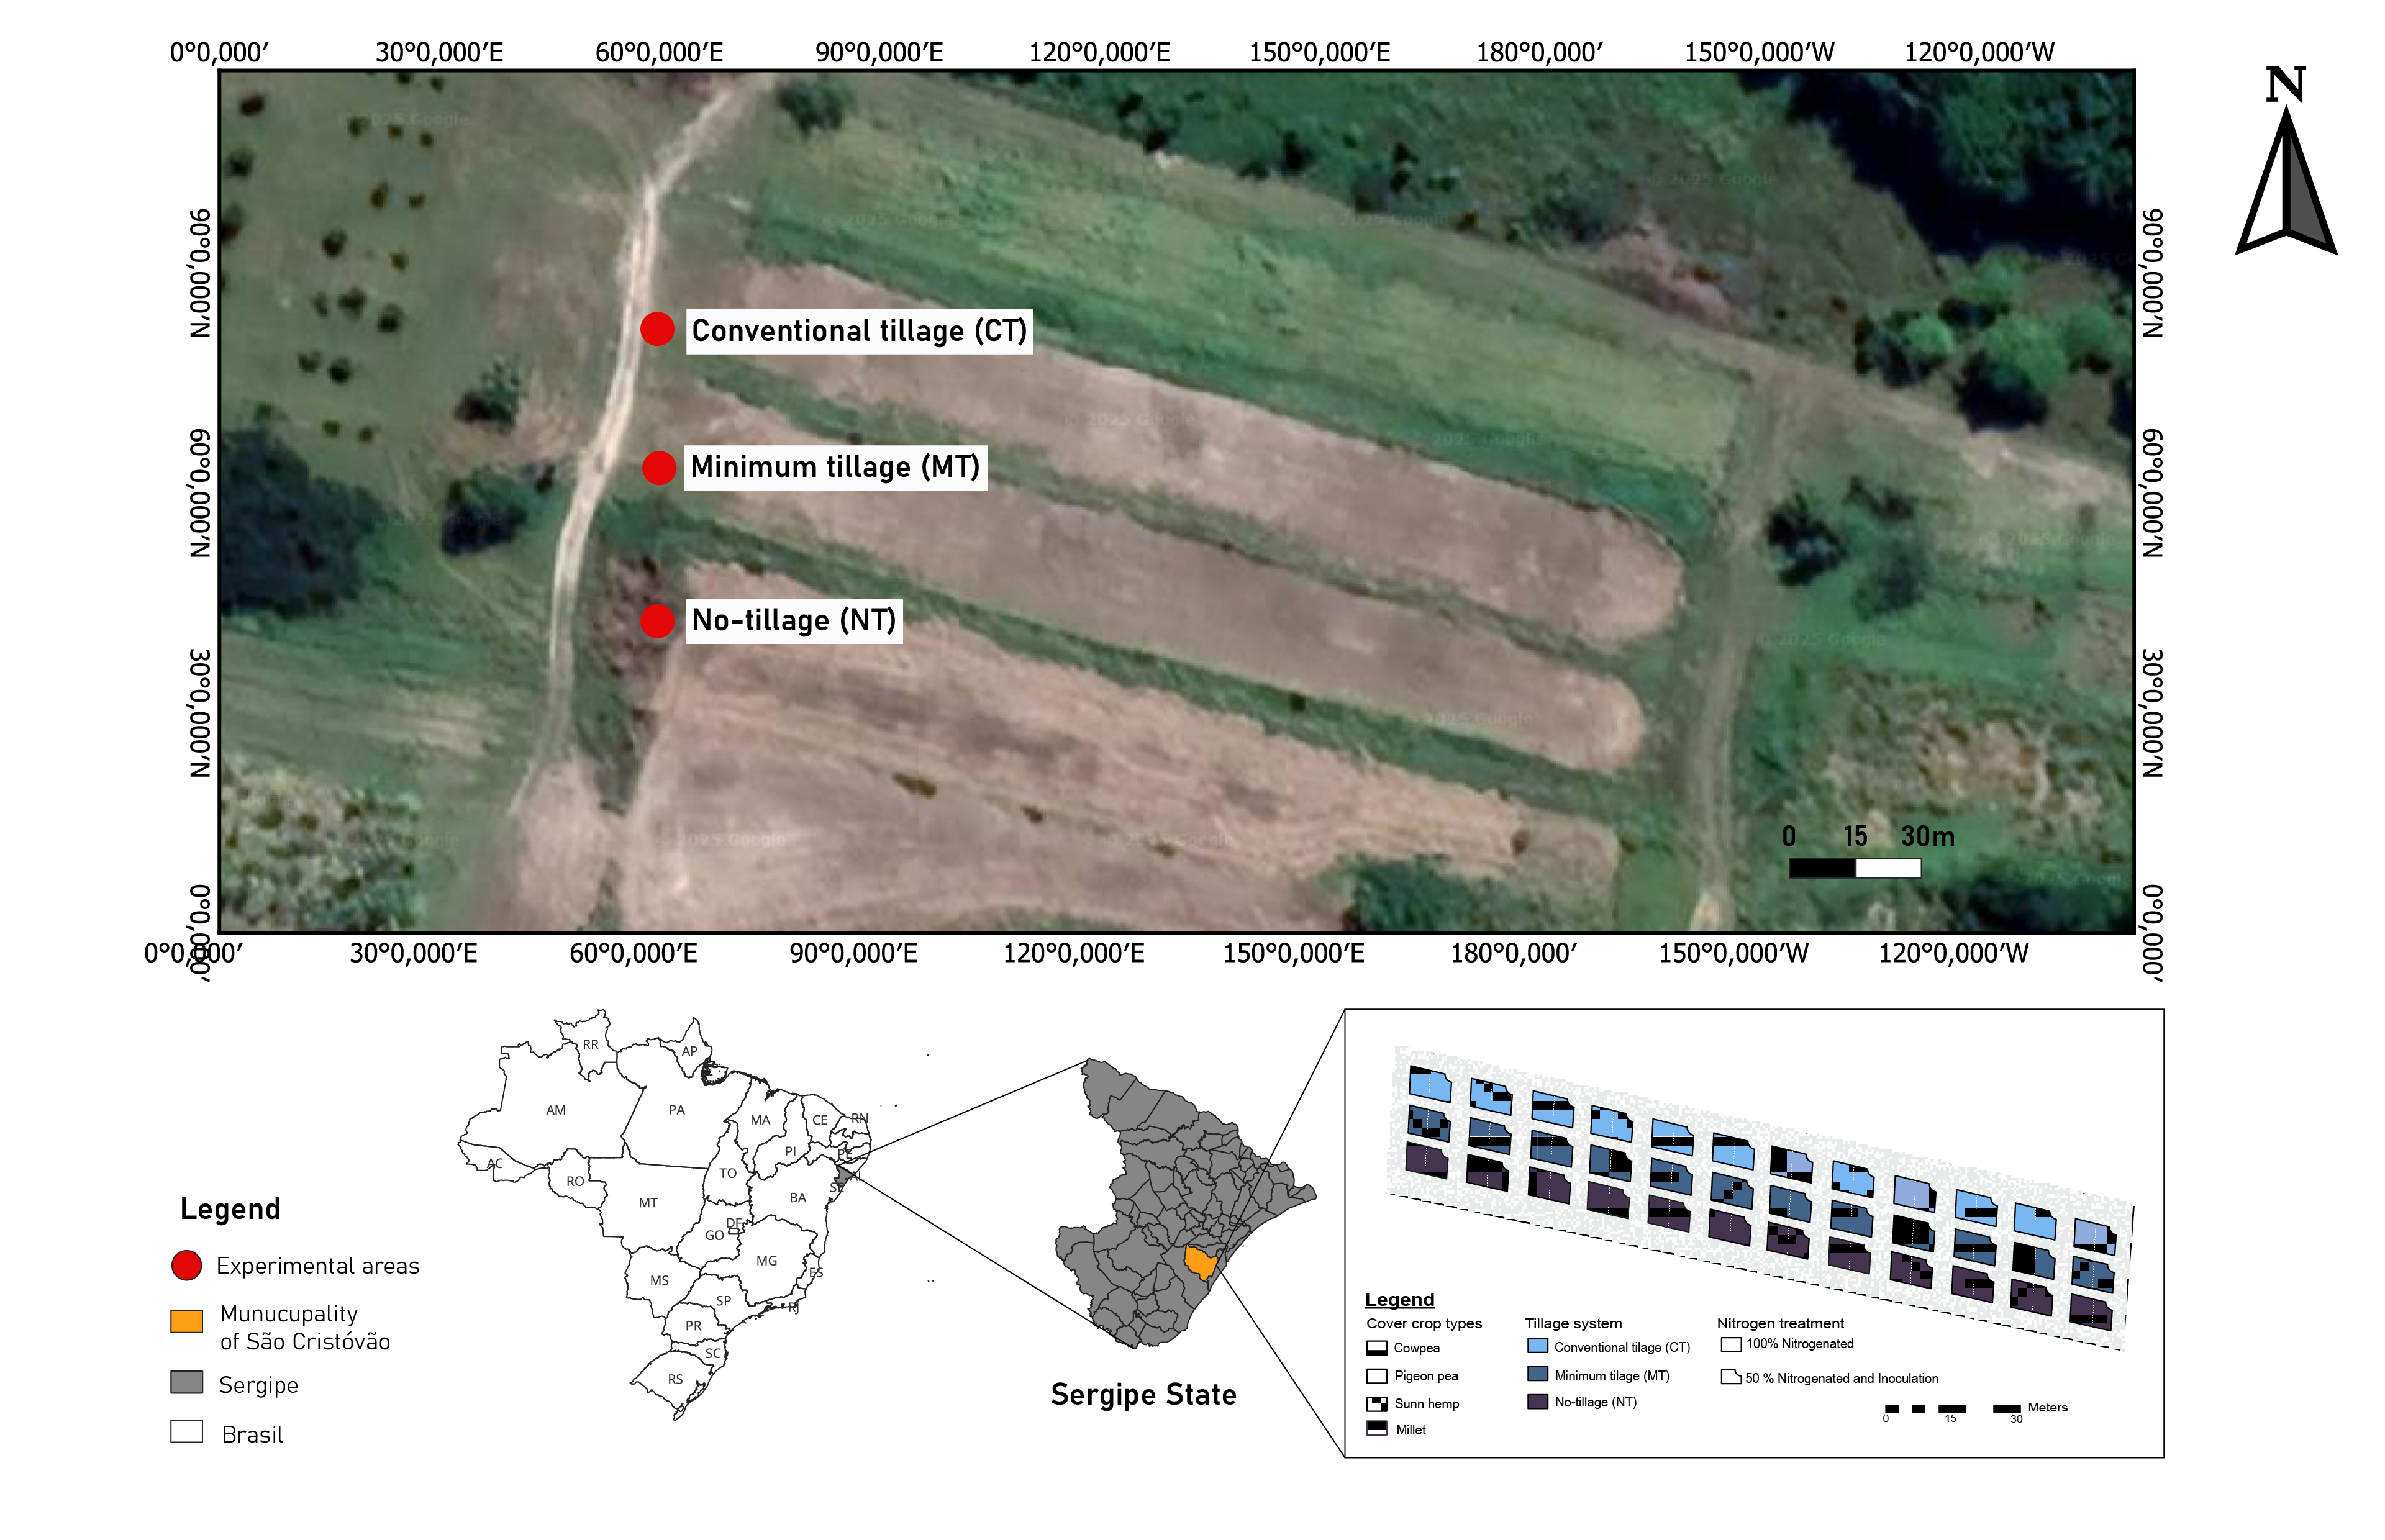
\includegraphics[width=0.85\textwidth]{../../2-DADOS/3-FIGURAS/fig_experimental_site.jpg}
\caption{Location and overview of the long-term experiment (established in 2001) at the Experimental Station of the Universidade Federal de Sergipe, municipality of S\~{a}o Crist\'{o}v\~{a}o, SE, Brazil, on a Typic Hapludult of the Coastal Tablelands.}\label{fig:site}
\end{figure}

Observations ($n = 108$) were collected in a factorial design combining three tillage systems (no-tillage, NT; conventional tillage, CT; and minimum tillage, MT) with four cover crop species (cowpea, \textit{Vigna unguiculata}; pearl millet, \textit{Pennisetum glaucum}; pigeon pea, \textit{Cajanus cajan}; and sunn hemp, \textit{Crotalaria juncea}), totaling 12 combinations with nine replicates each. The main crop \textit{Zea mays} L. (hybrid SHS7990 PRO3) was sown at 0.80\,m\,$\times$\,0.20\,m spacing ($\approx$\,54,000\,plants\,ha$^{-1}$), preceded by the cover crop sown manually 90 days prior. Conventional tillage consisted of disk plowing to 25\,cm followed by leveling harrow, minimum tillage employed only the leveling harrow, and no-tillage dispensed with mechanical soil disturbance.

With nine replicates per factorial cell ($3 \times 4 = 12$ combinations), the design totals $n = 108$ observations. The \textit{a posteriori} power analysis for the factorial ANOVA with $\alpha = 0.05$, medium effect size ($f = 0.25$), and $k = 12$ groups indicates statistical power $> 0.90$ for detecting differences among management combinations, meeting the threshold recommended by \cite{Mundform2005} for multivariate analyses. Sampling was restricted to the 0--0.20~m layer for operational reasons, since the cohesive layer in this Acrisol occurs between 0.25 and 0.45~m depth \citep{LimaNeto2010} and collection at greater depths would require trenches in all 108 plots, which was unfeasible in the context of a long-term experiment with 60~m$^2$ subplots. This restriction may underestimate physical differentiation among treatments that act on the cohesive layer (e.g., pivoting root of pigeon pea), constituting a recognized limitation of this study.

\subsection{Soil and plant indicators}\label{subsec:indicators}

Eighteen indicators spanning the physical soil, chemical, agronomic, and yield domains were measured (Table~\ref{tab:indicators}). Physical, agronomic, and yield indicators were obtained in the 2022 growing season of the present experiment; chemical indicators (pH, P, and K) were obtained from a complementary assessment conducted in the same experimental plots at 0--10\,cm depth and integrated into the dataset as means per design cell (tillage\,$\times$\,cover crop). Observed values (pH 4.1--5.7; P 35--93\,mg\,dm$^{-3}$; K 36--166\,mg\,dm$^{-3}$) are consistent with the range of variation reported for tropical Acrisols under fertilized systems \citep{Nabiollahi2020} and confer representativeness to the chemical fertility domain usually required in SQI protocols \citep{Andrews2002}. Soil pH was determined in a soil:water suspension (1:2.5) with a calibrated potentiometer (precision $\pm 0.02$), available P by Mehlich-1 with UV-Vis spectrophotometer reading at 725\,nm (analytical CV $< 5$\%), and available K by Mehlich-1 with flame photometer reading (analytical CV $< 4$\%). Soil organic carbon stock (SOC) was determined by modified Walkley-Black (CV $< 6$\%). The inclusion of the three chemical indicators required recalibration of the FIS membership functions (expansion of the universe of discourse), readjustment of RF hyperparameters (\texttt{mtry} recalculated to $\lfloor \sqrt{18} \rfloor = 4$) and MARS (forward/backward reprocessing), as well as re-specification of the CHEMICAL construct in PLS-SEM, so that all paradigms were re-estimated with the full 18-indicator vector.

\begin{table}[h]
\caption{Soil and plant indicators used in the benchmarking analysis.}\label{tab:indicators}
\begin{tabular*}{\textwidth}{@{\extracolsep\fill}llll}
\toprule
Domain & Indicator & Abbreviation & Unit \\
\midrule
\multirow{7}{*}{Physical soil}
  & Geometric mean diameter & GMD & mm \\
  & Mean weight diameter & MWD & mm \\
  & Bulk density & BD & Mg\,m$^{-3}$ \\
  & Residual moisture persistence & RMP & -- \\
  & Water-stable aggregates & WSA & \% \\
  & Soil organic carbon stock & SOC & Mg\,ha$^{-1}$ \\
  & Vegetation cover index & VCI & \% \\
\midrule
\multirow{3}{*}{Chemical soil}
  & pH in water (0--10\,cm) & pH & -- \\
  & Available phosphorus (0--10\,cm) & P & mg\,dm$^{-3}$ \\
  & Available potassium (0--10\,cm) & K & mg\,dm$^{-3}$ \\
\midrule
\multirow{4}{*}{Agronomic}
  & Plant height & PH & cm \\
  & Ear diameter & ED & mm \\
  & Ear length & EL & cm \\
  & Final stand & STAND & plants\,ha$^{-1}$ \\
\midrule
\multirow{4}{*}{Yield}
  & Total ears per hectare & TE & ears\,ha$^{-1}$ \\
  & Marketable ears per hectare & ME & ears\,ha$^{-1}$ \\
  & Marketable ear weight per hectare & MEW & kg\,ha$^{-1}$ \\
  & Architectural quality index & AQI & -- \\
\botrule
\end{tabular*}
\smallskip\noindent\textit{Note:} All indicators were normalized to the 0--10 scale prior to application of the fuzzy and ML paradigms. Chemical indicators were obtained from a complementary assessment in the same experimental area and integrated as means per design cell.
\end{table}

\subsection{Paradigm 1: ANOVA/GLM with minimum data set selection}\label{subsec:anova}

The classical approach was included because it represents the most widely used paradigm in the SQI literature and operates under additivity and monotonicity assumptions that serve as a baseline for gauging the informational gain of nonlinear methods. The variability-capture mechanism is restricted to linear variance decomposition by PCA eigenvalues, which implies that higher-order interactions and threshold effects among soil domains remain in the unexplained residual.

Generalized linear models (GLM) were fitted for each indicator following the protocol of \cite{Andrews2002} according to
\begin{equation}
Y_{ijk} = \mu + \alpha_i + \beta_j + (\alpha\beta)_{ij} + \varepsilon_{ijk}
\label{eq:glm}
\end{equation}
where $\alpha_i$ represents the effect of the tillage system ($i = 1, 2, 3$), $\beta_j$ the effect of the cover crop species ($j = 1, \ldots, 4$), $(\alpha\beta)_{ij}$ their interaction, and $\varepsilon_{ijk}$ the residual error. Type~II ANOVA was processed with the \texttt{car} package. Multiple comparisons among means were performed using estimated marginal means (\texttt{emmeans}) with Tukey adjustment.

Minimum data set (MDS) selection was conducted via PCA. Indicators with factor loadings exceeding 0.70 on each retained component were identified, and among correlated indicators within each component, the one with the highest communality was retained. The linear SQI was computed as
\begin{equation}
\text{SQI}_{\text{ANOVA}} = \sum_{i=1}^{k} w_i \cdot S_i
\label{eq:sqi_anova}
\end{equation}
where $w_i$ corresponds to the PCA-derived eigenvalue weight and $S_i$ to the normalized score of each indicator. Residual normality of the GLM was assessed by the Shapiro-Wilk test and homoscedasticity by the Levene test (\texttt{car} package). Indicators whose residuals violated the normality assumption ($p < 0.05$) were Box-Cox transformed prior to ANOVA; when transformation did not normalize residuals, nonparametric ANOVA (Kruskal-Wallis) followed by Dunn's test with Bonferroni adjustment was employed.

\subsection{Paradigm 2: Fuzzy inference system}\label{subsec:fuzzy}

Fuzzy inference was selected for its ability to accommodate the gradual transition among soil quality classes without imposing crisp boundaries on continuous indicators. The mechanism operates through overlapping membership functions that assign partial degrees of association to each linguistic category, preserving the inherent uncertainty at the boundary between ``low'' and ``medium'' or ``medium'' and ``high'' that additive scoring eliminates by discretizing indicators into 0--1 scores. Threshold effects that linear combination compresses can thus be captured by the rule base without prior parametric specification.

A Mamdani-type fuzzy inference system \citep{Mamdani1975} was constructed following the framework of \cite{Torbert2008}. Each of the 15 original indicators was fuzzified into three linguistic categories (low, medium, high) with triangular and, separately, Gaussian membership functions. Triangular functions were defined as
\begin{equation}
\mu_A(x) = \max\left(\min\left(\frac{x-a}{b-a},\; \frac{c-x}{c-b}\right),\; 0\right)
\label{eq:trimf}
\end{equation}
where $a$, $b$, and $c$ delimit the support and peak of the fuzzy set. Gaussian functions followed
\begin{equation}
\mu_A(x) = \exp\left(-\frac{(x-c)^2}{2\sigma^2}\right)
\label{eq:gaussmf}
\end{equation}

The rule base was derived from expert knowledge and defuzzification was performed using the centroid method. The output, designated the Integrated Soil Performance and Conservation Index (IPACSA), was computed on the 0--10 scale with the \texttt{FuzzyR} package.

\subsection{Paradigm 3: PLS-SEM structural equation modeling}\label{subsec:sem}

PLS-SEM was included because it enables the specification of directional relationships among soil domains (physical, chemical, agronomic, yield) as latent constructs, testing explicit causal hypotheses about the soil--plant--yield chain. The capture mechanism resides in the estimation of path coefficients that weight the relative contribution of each domain to yield, while the formative specification (Mode~B) allows indicators such as pH, P, and K to act as determinants of fertility rather than as reflective manifestations of a latent factor. This flexibility distinguishes PLS-SEM from the other paradigms by incorporating a theoretical structure into the aggregation, although the linearity of the structural paths limits the capture of higher-order interactions.

A hierarchical PLS path model was specified with four first-order latent constructs (PHYSICAL, CHEMICAL, AGRONOMIC, and YIELD) and a second-order construct, SQI. The structural model specified directional paths according to
\begin{equation}
\text{SQI}_{\text{PLS}} = \gamma_1 \cdot \eta_{\text{PHYS}} + \gamma_2 \cdot \eta_{\text{CHEM}} + \gamma_3 \cdot \eta_{\text{AGRO}} + \gamma_4 \cdot \eta_{\text{YIELD}} + \zeta
\label{eq:plssem}
\end{equation}
Indicators such as bulk density (BD) and ear production (MEW, ME) act as causes (rather than reflections) of their respective constructs, implying formative relationships. For this reason, the model adopted a mixed specification (Mode~A for reflective indicators and Mode~B for formative indicators), as recommended by \cite{Hair2019}. Four indicators with VIF\,$> 5$ (MWD, RMP, BD, ME) were excluded prior to estimation to avoid correlation matrix singularity, resulting in 14 indicators distributed among the four first-order constructs: PHYSICAL (Mode~B: GMD, SOC, WSA, VCI), CHEMICAL (Mode~B: pH, P, K), AGRO (Mode~B: PH, ED, EL, STAND), and YIELD (Mode~A: TE, MEW, PROD). Mode~B validation followed criteria of outer weight significance and absence of residual multicollinearity.

Estimation followed a two-stage approach with the \texttt{seminr} package \citep{Ray2022}. Overall model quality was assessed by the SRMR (Standardized Root Mean Square Residual), with an acceptance threshold of $< 0.08$ \citep{Hair2019}, and by the Goodness of Fit (GoF) as the geometric mean of average communalities and average $R^2$ of endogenous constructs. For formative constructs (Mode~B), a redundancy test by correlation between the formative score and a global reflective indicator was applied, verifying convergent validity when $r > 0.70$. In the first stage, the four first-order constructs (PHYSICAL, CHEMICAL, AGRO, YIELD) were iteratively estimated, with structural paths PHYSICAL$\to$YIELD, CHEMICAL$\to$YIELD, and AGRO$\to$YIELD. In the second stage, the latent scores of the four constructs were subjected to PCA, and the first principal component was adopted as SQI$_{\text{PLS}}$, scaled to the 0--10 interval. Confidence intervals for path coefficients were obtained through 5,000-resample bootstrap.

\subsection{Paradigm 4: MARS with ablation analysis}\label{subsec:mars}

MARS was selected for its ability to identify response discontinuities through hinge functions that segment the predictor space into locally linear regions, without requiring prior discretization or specification of the number or position of thresholds. The nonlinearity-capture mechanism resides in the automatic selection of adaptive knots by the forward addition and backward pruning algorithm, which approximate relationships whose curvature varies along the indicator range.

MARS models \citep{Friedman1991} were fitted with the \texttt{earth} package \citep{Milborrow2023} to capture nonlinear relationships between indicators and a target variable (yield or composite SQI). The model selected basis functions through forward stepwise addition and backward pruning according to
\begin{equation}
\hat{f}(x) = \beta_0 + \sum_{m=1}^{M} \beta_m \prod_{k=1}^{K_m} h_{km}(x_{v(k,m)})
\label{eq:mars}
\end{equation}
where $h_{km}$ are hinge functions of the form $\max(0, x - t)$ or $\max(0, t - x)$.

Variable importance was assessed through ablation analysis, in which each indicator was sequentially removed and the mean absolute rank shift quantified the impact on the predicted SQI.

Indicators whose ablation score exceeded a predefined threshold were classified as irreplaceable for the index. The adequacy of the adaptive knots was verified through a Residuals $\times$ Fitted Values plot and the Breusch-Pagan test for heteroscedasticity (\texttt{lmtest} package); the absence of systematic pattern in the residuals and $p > 0.05$ in the BP test confirm that the hinge functions adequately capture the variance structure of the data. Additionally, global variable importance was estimated via SHAP (SHapley Additive exPlanations) values with the \texttt{DALEX} package, enabling direct comparison with RF importance metrics and interpretive alignment across paradigms.

\subsection{Paradigm 5: Random Forest regression}\label{subsec:rf}

RF \citep{Breiman2001} was included for its ability to capture high-order interactions and nonlinearities through recursive partitioning of the predictor space in an ensemble of independent decision trees. The mechanism operates through bootstrap aggregation (bagging) of multiple trees trained on random subsets of observations and variables, which reduces prediction variance and provides internal error estimates (OOB) that dispense with explicit train/test partitioning.

Random Forest models were trained with the \texttt{randomForest} package using 500 trees, $\lfloor \sqrt{q} \rfloor = 5$ variables randomly sampled at each split, and minimum terminal node size equal to~5. The choice of $\text{mtry} = \lfloor \sqrt{q} \rfloor$ instead of $\lfloor q/3 \rfloor$ reduces inter-tree correlation and confers greater ensemble stability when the $n/q$ ratio is moderate ($\approx 6.0$). Convergence of the out-of-bag error (OOB-MSE) was verified through the OOB-MSE $\times$ number-of-trees curve, and OOB error estimates provided an internal validation metric. Variable importance was quantified through two complementary approaches, the percentage increase in mean squared error (\%IncMSE) after permutation of each predictor and global SHAP values obtained with the \texttt{DALEX} package (500 permutations).

Ninety-five percent confidence intervals for SQI predictions were estimated using the infinitesimal jackknife method \citep{Wager2014} implemented in the \texttt{randomForestCI} package. In addition to $R^2_{\text{OOB}}$, OOB-RMSE was reported in original units of the 0--10 scale to allow direct interpretation of predictive error magnitude. The predicted SQI was defined as
\begin{equation}
\text{SQI}_{\text{RF}} = \frac{1}{B}\sum_{b=1}^{B} T_b(\mathbf{x})
\label{eq:rf}
\end{equation}
where $T_b$ corresponds to the prediction of tree $b$ for observation $\mathbf{x}$.

\subsection{Inter-paradigm concordance assessment}\label{subsec:concordance}

The five paradigms generate SQI values on different scales. Prior to comparison, all SQI vectors were standardized through inverse-normal rank transformation \citep{Blom1958} according to
\begin{equation}
z_i = \Phi^{-1}\!\left(\frac{r_i - 0.5}{n}\right)
\label{eq:blom}
\end{equation}
where $r_i$ is the rank of observation $i$ and $\Phi^{-1}$ the quantile function of the standard normal distribution. This transformation preserves the original ordering and places all paradigms on a standard Gaussian scale, eliminating distortions arising from domain differences (0--1 vs.\ 0--10 vs.\ factor scores).

The comparison across mathematical families aimed to isolate the variance attributable to paradigm choice and estimate the false-positive rate that inadequate models may generate. Kendall's coefficient of concordance ($W$) assessed consistency among the five simultaneous rankings (permutation test with 10,000 repetitions). The intraclass correlation coefficient, ICC(2,1) \citep{ShroutFleiss1979}, estimated absolute agreement. Additionally, \cite{Gwet2008}'s AC2 coefficient corrected for chance-expected agreement (\texttt{irrCAC} package).

To delimit ranges in which paradigm switching would alter management classification, Bland--Altman analysis \citep{BlandAltman1986} quantified limits of agreement through systematic bias plots ($\text{SQI}_A - \text{SQI}_B$) with limits at $\pm 1.96$ standard deviations. Additionally, a Spearman correlation matrix ($\rho$) quantified correlations among the standardized SQI vectors. A consensus meta-SQI was computed as the mean of ranks (Borda count) across the five paradigms \citep{Lin2010}.

The test of $H_2$ (higher concordance among nonlinear paradigms) was conducted using paired Wilcoxon on Fisher-$Z$-transformed $\rho$ values, comparing the subset of nonlinear$\times$nonlinear pairs with linear$\times$nonlinear pairs.

\subsection{Sample-size sensitivity}\label{subsec:sensitivity}

Concordance sensitivity to sample size was assessed through stratified Monte Carlo simulation, aiming to establish the sample-size threshold above which inter-paradigm concordance stabilizes at acceptable levels. The full dataset ($n = 108$) was subsampled at five levels ($n = 15$, 30, 50, 75, 100) with 1,000 iterations per level. At each iteration, sampling was stratified by factorial design cell (tillage $\times$ cover crop), preserving original proportionality and preventing casual imbalance from artificially inflating inter-paradigm variance. The random seed of each iteration was stored for reproducibility. In each subsample, the five paradigms were reprocessed and Kendall's $W$ recalculated, enabling assessment of concordance dependence on sample size. The test of $H_3$ (log-linear relationship between $W$ and $n$) was conducted through GLS regression of $\bar{W}$ on $\log(n)$ with correlation structure for paired observations, identifying the threshold above which sample-size increments no longer reduce concordance variability among rankings.

%% ================================================================
%%                    SECTION 4: RESULTS AND DISCUSSION
%% ================================================================
\section{Results and Discussion}\label{sec:results_discussion}

\subsection{Predictive performance and variable importance}\label{subsec:performance}

The Random Forest model explained 97.1\% of SQI variance by the out-of-bag error ($R^2_{\text{OOB}} = 0.971$; OOB-RMSE $= 0.54$ on the 0--10 scale), with OOB-MSE stabilization from approximately 200 trees onward and 95\% confidence intervals with a mean width of 1.18 units on the 0--10 scale, indicating precision compatible with the between-replicate variability within each factorial cell.

Permutation importance (\%IncMSE) identified yield- and agronomic-domain variables as the primary predictors (Fig.~\ref{fig:importance}), with total ears per hectare (23.9\%), final stand (21.4\%), marketable ears (14.2\%), and productivity (14.1\%) accounting for more than 73\% of accumulated importance. The three chemical-domain indicators occupied an intermediate tier, with K (10.5\%), P (9.6\%), and pH (7.4\%) individually surpassing all physical-domain indicators except VCI (12.3\%). Physical soil indicators (GMD, MWD, WSA, BD) each contributed less than 7\%.

Global SHAP values, obtained through 500 permutations via DALEX, corroborated this hierarchy, with reduced dispersion for the highest-importance variables \citep{Lundberg2017,Shahriari2023}. Incorporation of the chemical indicators did not alter the hierarchy of the remaining domains but established a fourth importance tier between the productive/agronomic and physical components, which is consistent with the mediating role of chemical fertility in the soil--plant relationship documented by \cite{Nabiollahi2020} in rainfed systems. \cite{Zhao2022}, in a long-term factorial experiment on a Mollisol in China, observed that chemical attributes responded more rapidly to management than physical indicators, which required more than 15 years to attain statistically detectable differences between rotations with and without cover crops. In Acrisols of the Coastal Tablelands, the cohesive subsurface layer may amplify this asymmetry by constraining physical differentiation among treatments within the sampled layer (0--0.20~m), channeling most of the explainable variance to agronomic and chemical indicators situated above the mechanical restriction.

\begin{figure}[ht]
\centering
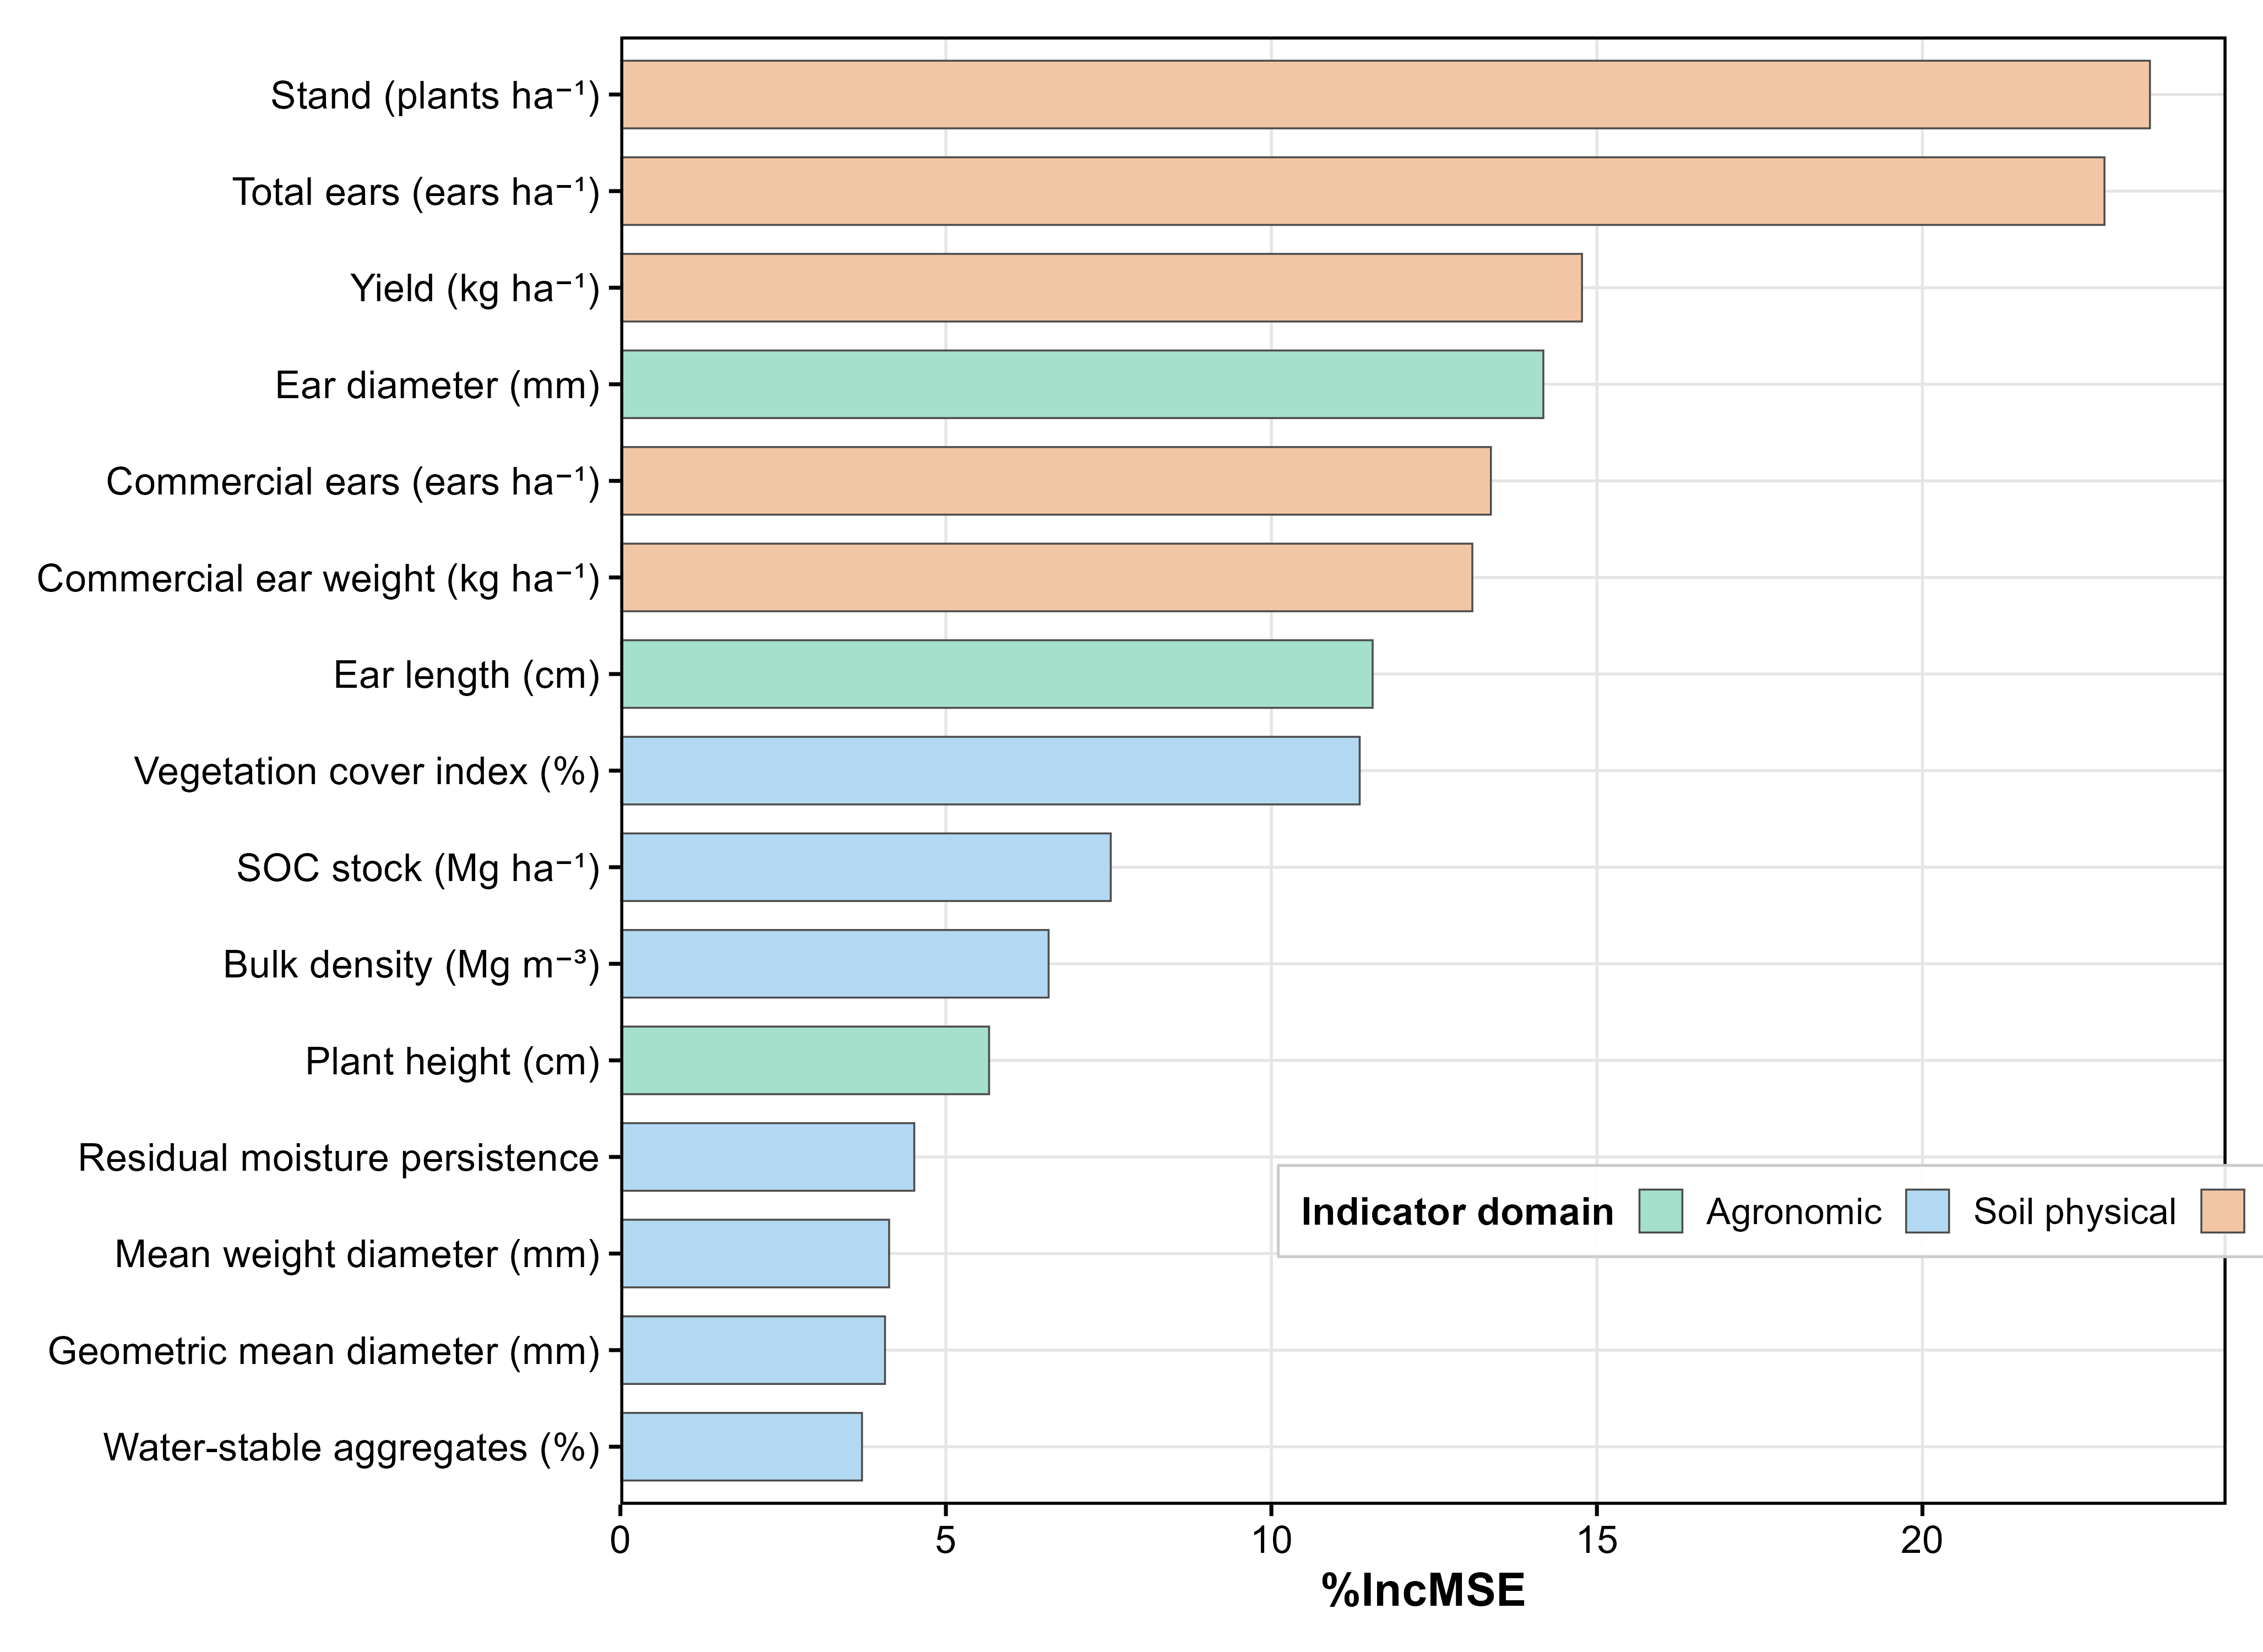
\includegraphics[width=0.75\textwidth]{../../2-DADOS/3-FIGURAS/fig_rf_importance.png}
\caption{Variable importance by permutation (\%IncMSE) in the RF model.}\label{fig:importance}
\smallskip\noindent\textit{Note:} Bars colored by indicator domain.
\end{figure}

Partial dependence curves (Fig.~\ref{fig:pdp}) reveal that total ears per hectare and plant stand exhibit a sigmoidal response on the RF-predicted SQI, with a transition threshold between normalized values 4 and 6, above which the marginal effect stabilizes at an asymptotic plateau. Ear diameter and productivity, in turn, display a monotonically increasing response with lower saturation intensity, suggesting a quasi-linear contribution to the integrated score \citep{Friedman2001}. This threshold pattern may reflect the compensatory effect among cover crop species in an Acrisol with a cohesive layer, where productivity gains stabilize above a certain stand level while morphological attributes maintain a gradual dose--response relationship \citep{Assuncao2023}. \cite{Moitinho2020}, assessing arbuscular mycorrhizal fungi under no-tillage with corn/cover crop rotation in a Red Acrisol, observed that pigeon pea and sunn hemp promoted greater spore abundance and aggregate stability index than monoculture grasses, suggesting that rhizospheric biological mediation may contribute to the coupling between physical quality and productive response captured by the PDPs.

\begin{figure}[ht]
\centering
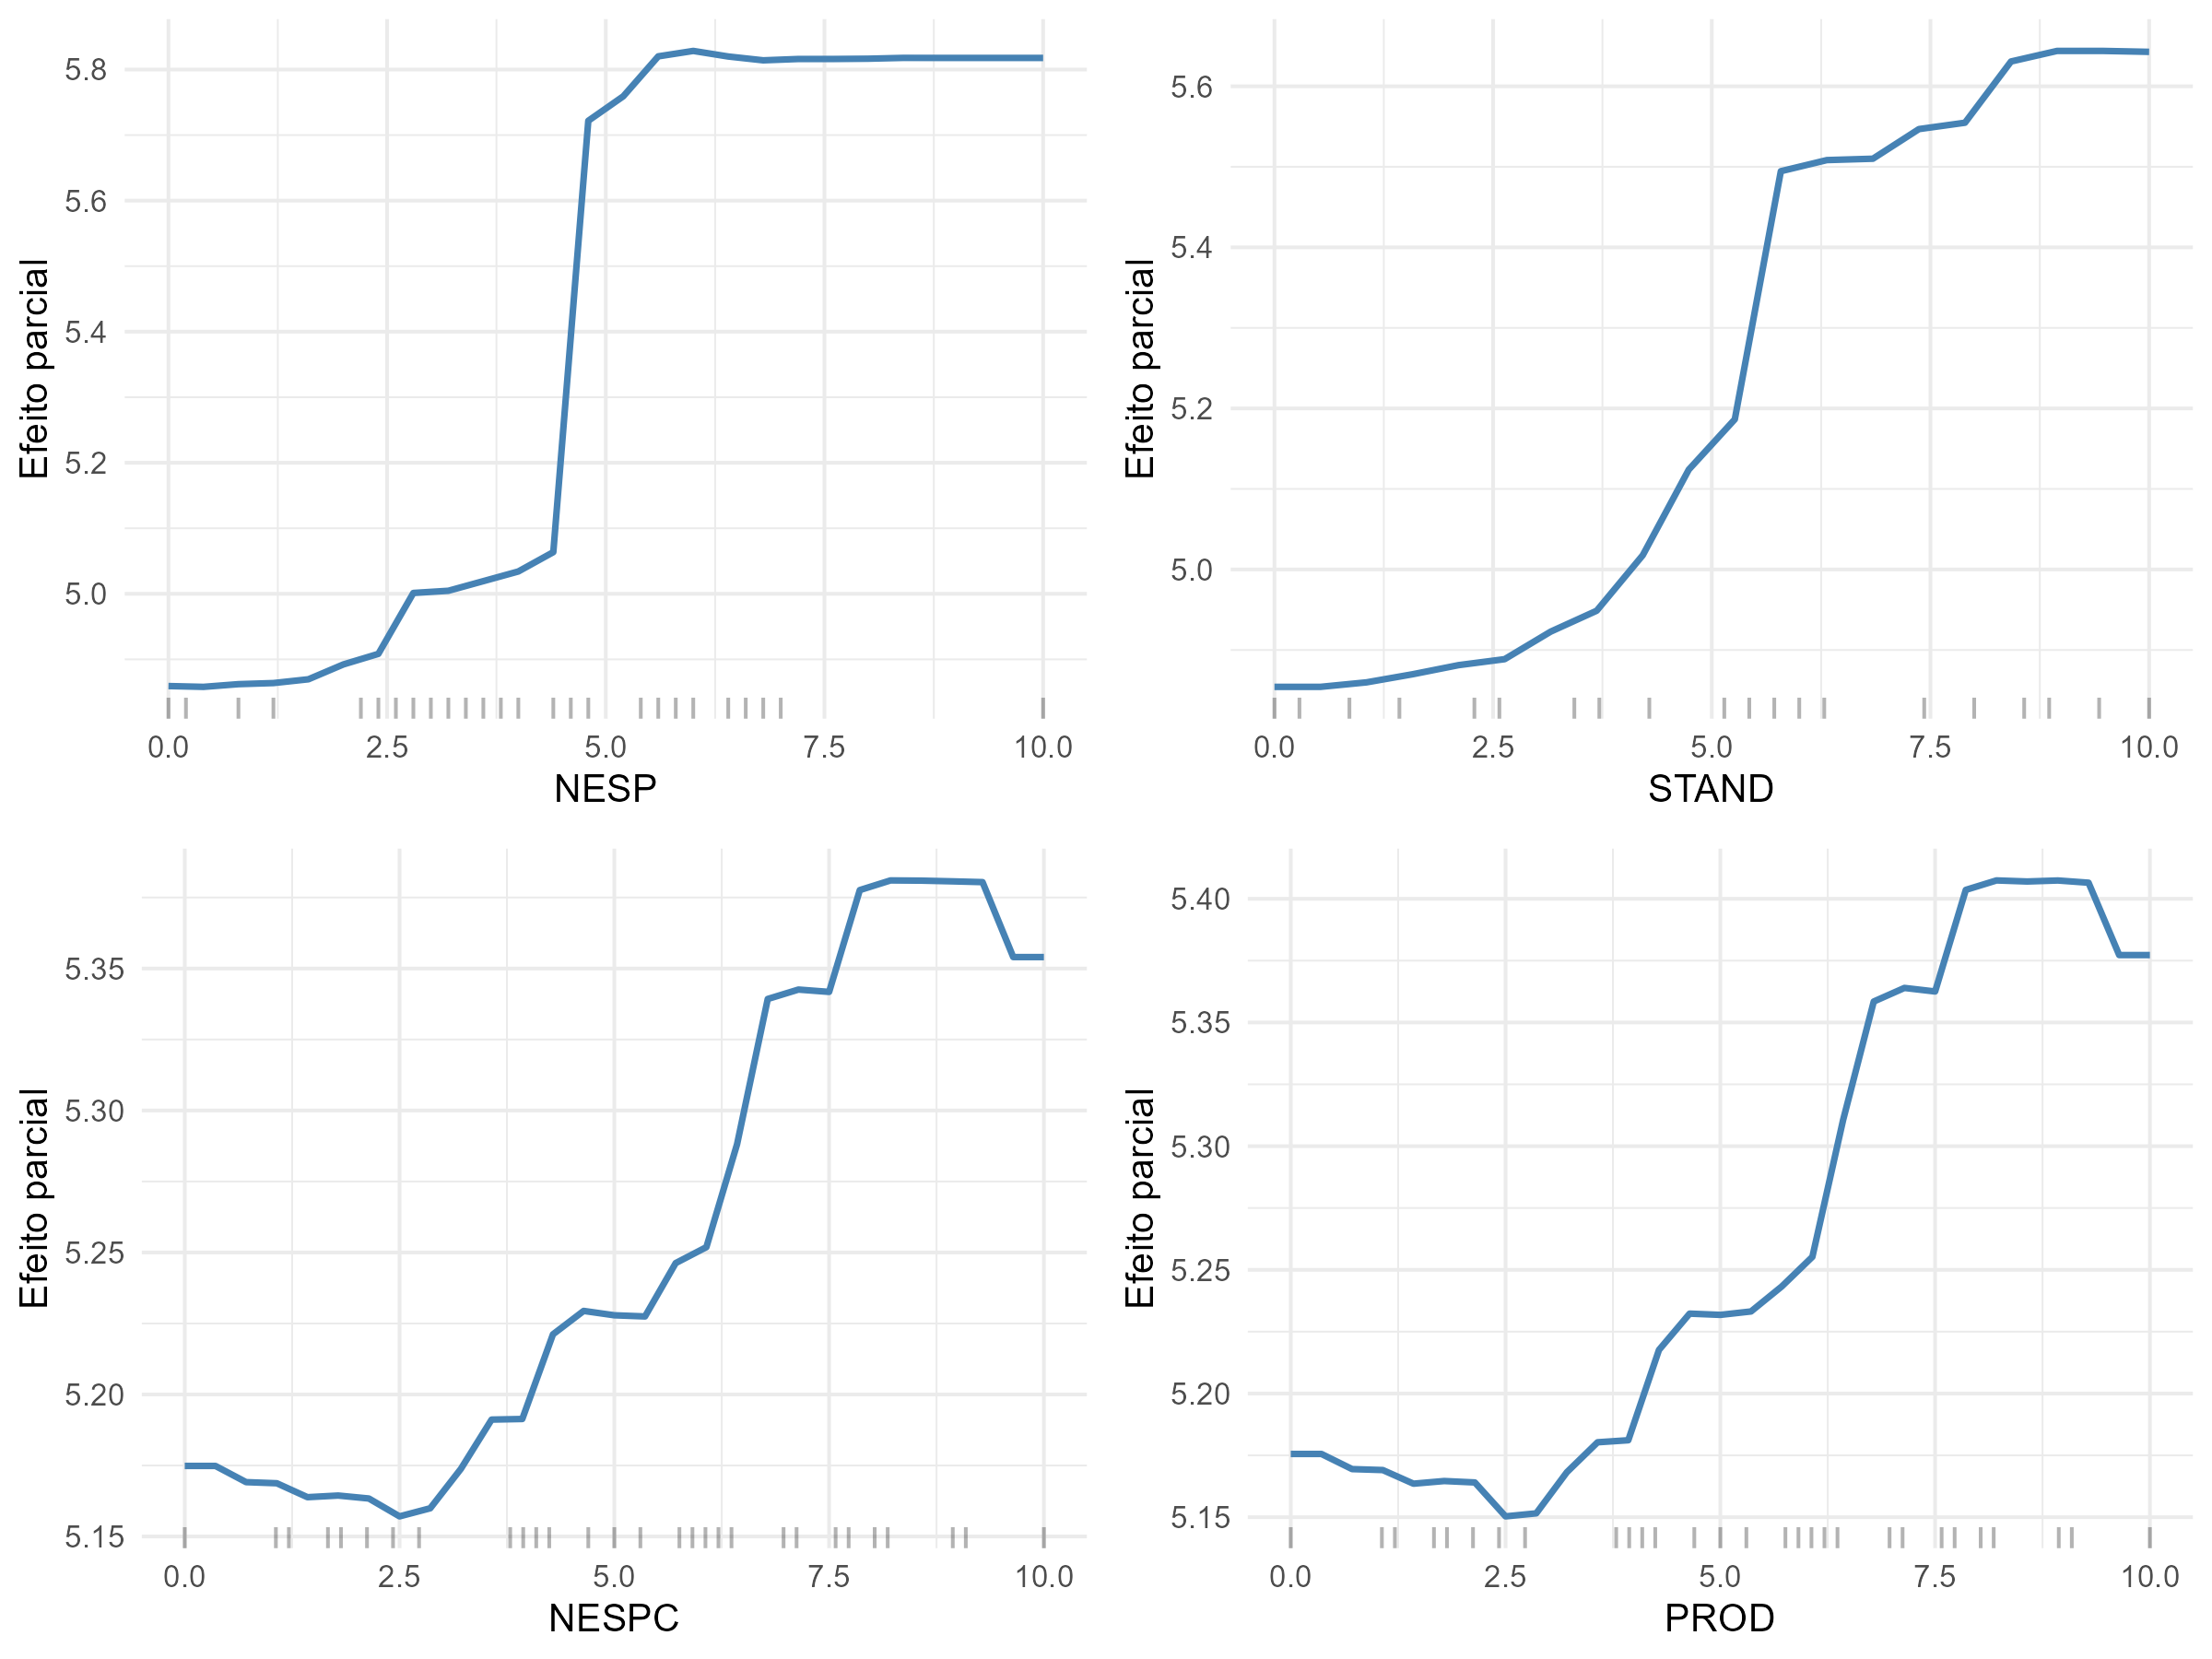
\includegraphics[width=\textwidth]{../../2-DADOS/3-FIGURAS/fig_pdp_top4.png}
\caption{Partial dependence curves for the four most important indicators in the RF model.}\label{fig:pdp}
\smallskip\noindent\textit{Note:} Horizontal axis, normalized value (0--10); vertical axis, partial effect on the predicted SQI. Rug plots indicate the marginal data distribution.
\end{figure}

In the PLS-SEM model with four constructs, AGRO explained the largest share of YIELD variance ($\gamma = 0.717$, $p < 0.001$, 95\% bootstrap CI: 0.599--0.826), whereas the PHYSICAL$\to$YIELD path did not reach significance ($\gamma = -0.056$, $p = 0.674$). The new CHEMICAL construct exhibited a negative and marginally significant coefficient ($\gamma = -0.168$, $p = 0.077$), which may indicate an inverse relationship between chemical fertility and yield in this system. This pattern may reflect nutrient dilution in plots with higher biomass production, where the proportionally greater absorption of P and K reduces residual soil concentrations \citep{Berriel2023}, although the antagonism between available P and nutrient-use efficiency under conservation management with continuous legume inputs may also contribute to the negative coefficient \citep{Nabiollahi2018}. Additionally, the cohesive layer present between 0.25 and 0.45~m in this Acrisol restricts root exploration and concentrates absorption in the sampled layer (0--0.10~m), which may amplify the apparent negative correlation between residual fertility and yield. Confirmation of this mechanism requires depth-stratified sampling (0--0.10 vs.\ 0.10--0.20 vs.\ 0.20--0.40~m) and analysis of X-ray computed tomography images or thin sections that would enable visualization of the structural discontinuity of the cohesive layer and its influence on root distribution, constituting a direction for future investigations.

VIF values for the CHEMICAL construct indicators were satisfactory (pH\,=\,1.08; P\,=\,1.41; K\,=\,1.32), with phosphorus exhibiting the highest outer weight (0.878), followed by pH (0.355) and K ($-0.237$). The structural model $R^2$ was 0.640 (Adj.\,$R^2$\,=\,0.630). The second-order construct, obtained from the first principal component of the four latent scores, captured 59.5\% of total variance, with loadings of 0.31 (PHYSICAL), $-0.49$ (CHEMICAL), 0.59 (AGRO), and 0.57 (YIELD). The negative weight of CHEMICAL on PC1 reflects the negative correlation between fertility and agronomic performance ($r_{\text{CHEM-AGRO}} = -0.52$), which may signal a nutrient dilution effect in plots with higher biomass productivity \citep{Berriel2023}. The presence of the cohesive layer between 0.25 and 0.45~m in this Acrisol \citep{LimaNeto2010} may act as a moderator of this relationship by restricting the soil volume explored by roots and concentrating both nutrient absorption and the response of physical indicators in the sampled surface layer, artificially amplifying the negative correlation between residual fertility and yield.

The five paradigms produced SQI distributions with distinct amplitudes and dispersions. FIS, MARS, and RF exhibited similar means (5.24 on the 0--10 scale), while SQI$_{\text{PLS}}$ (mean\,$=$\,4.51) and SQI$_{\text{ANOVA}}$ (mean\,$=$\,3.72) occupied broader ranges (0--10), reflecting the linearity and dimensional reduction imposed by these paradigms.

\subsection{Inter-paradigm concordance and meta-SQI}\label{subsec:concordance_disc}

Kendall's concordance coefficient ($W = 0.825$, $\chi^2 = 441.2$, $p < 2.2 \times 10^{-16}$) supported $H_1$ \citep{Legendre2012}, indicating significant concordance among the five simultaneous rankings. The permutation test (10,000 repetitions) corroborated this result ($p < 0.0001$). The ICC(2,1) of 0.742 (95\% CI: 0.679--0.801) indicates substantial absolute agreement, close to the 0.75 threshold generally considered ``good'' in reliability applications \citep{Koo2016}. Gwet's AC1 coefficient, calculated on SQI value quintiles, was 0.405, a more conservative value reflecting penalization for marginal chance-expected agreement. The addition of three chemical indicators raised $W$ from 0.81 (model with 15 indicators) to 0.83 and ICC from 0.72 to 0.74, suggesting that incorporation of the chemical fertility domain reduced inter-paradigm divergence by providing additional discriminating information in the between-plot dimension.

The Spearman correlation matrix revealed a two-block structure (Table~\ref{tab:spearman}). FIS, MARS, and RF formed a nearly indistinguishable block ($\rho > 0.993$ between any pairs), while ANOVA and PLS-SEM converged with each other ($\rho = 0.832$) and exhibited moderate correlations with the nonlinear block ($\rho = 0.649$--$0.682$). The Wilcoxon test did not support $H_2$ ($W = 14$, $p = 0.381$), because the incorporation of chemical indicators raised correlations between ANOVA and the nonlinear paradigms ($\bar{\rho}_{\text{Lin-NL}} = 0.712$) relative to the 15-indicator model ($\bar{\rho}_{\text{Lin-NL}} = 0.642$), reducing the difference relative to the mean among nonlinear pairs ($\bar{\rho}_{\text{NL-NL}} = 0.827$). This result indicates that chemical-domain indicators contributed to homogenizing the information captured by the different paradigms, attenuating the advantage that nonlinear methods exhibited when the dataset contained only physical and agronomic indicators \citep{Ye2022}.

\begin{table}[ht]
\caption{Spearman correlation matrix ($\rho$) among the five SQI paradigms after Blom transformation.}\label{tab:spearman}
\begin{tabular*}{\textwidth}{@{\extracolsep\fill}lccccc}
\toprule
 & ANOVA & Fuzzy & PLS-SEM & MARS & RF \\
\midrule
ANOVA   & 1.000 & 0.676 & 0.832 & 0.656 & 0.682 \\
Fuzzy   &       & 1.000 & 0.663 & 0.994 & 0.995 \\
PLS-SEM &       &       & 1.000 & 0.649 & 0.668 \\
MARS    &       &       &       & 1.000 & 0.993 \\
RF      &       &       &       &       & 1.000 \\
\botrule
\end{tabular*}
\end{table}

Bland--Altman limits of agreement \citep{BlandAltman1986} (Table~\ref{tab:blandaltman}) quantitatively reinforced this two-block structure. LoA between pairs within the FIS-MARS-RF block ranged from $\pm 0.37$ (Fuzzy vs.\ RF) to $\pm 0.43$ (MARS vs.\ RF) on the Blom scale, suggesting practical interchangeability. In contrast, pairs involving ANOVA or PLS-SEM exhibited LoA from $\pm 1.25$ (ANOVA vs.\ PLS) to $\pm 1.77$ (ANOVA vs.\ MARS), indicating that substituting the linear paradigm with any nonlinear alternative may alter individual ranking positions.

\begin{table}[ht]
\caption{Bland--Altman analysis summary between paradigm pairs (Blom scale).}\label{tab:blandaltman}
\begin{tabular*}{\textwidth}{@{\extracolsep\fill}lcccc}
\toprule
Pair & $\bar{d}$ & $s_d$ & Lower LoA & Upper LoA \\
\midrule
Fuzzy vs RF    & 0.00 & 0.188 & $-$0.368 & 0.368 \\
Fuzzy vs MARS  & 0.00 & 0.217 & $-$0.426 & 0.426 \\
MARS vs RF     & 0.00 & 0.220 & $-$0.431 & 0.431 \\
PLS vs Fuzzy   & 0.00 & 0.868 & $-$1.701 & 1.701 \\
PLS vs MARS    & 0.00 & 0.902 & $-$1.768 & 1.768 \\
PLS vs RF      & 0.00 & 0.866 & $-$1.698 & 1.698 \\
ANOVA vs PLS   & 0.00 & 0.638 & $-$1.250 & 1.250 \\
ANOVA vs Fuzzy & 0.00 & 0.878 & $-$1.721 & 1.721 \\
ANOVA vs MARS  & 0.00 & 0.902 & $-$1.769 & 1.769 \\
ANOVA vs RF    & 0.00 & 0.861 & $-$1.687 & 1.687 \\
\botrule
\end{tabular*}
\smallskip\noindent\textit{Note:} $\bar{d}$, mean difference; $s_d$, standard deviation of the difference; LoA, limits of agreement ($\pm 1.96\,s_d$).
\end{table}

\clearpage

Practical interchangeability within the nonlinear block is confirmed by the homogeneous dispersion of the Fuzzy--RF pair within the $\pm 0.37$ band along the means axis, with points distributed symmetrically around zero difference and no proportional trend with SQI level. The ANOVA--Fuzzy pair, in contrast, displays a fan-shaped pattern suggesting proportional bias relative to the SQI level \citep{Giavarina2015}, with increasing disagreement toward higher Blom-scale values, indicating that linear compression progressively underestimates quality as the integrated score rises.

The PLS--RF pair occupies an intermediate position (LoA\,$\approx \pm 1.70$), with apparent heteroscedasticity at extreme values signaling more pronounced disagreement for management combinations with lower quality (Fig.~\ref{fig:ba_panel}). This concordance gradient, from the interchangeability of the nonlinear block to the systematic divergence of linear paradigms, reinforces that the choice of analytical family, rather than the internal parameterization of each algorithm, governs the degree of concordance among SQI rankings.

\begin{figure}[ht]
\centering
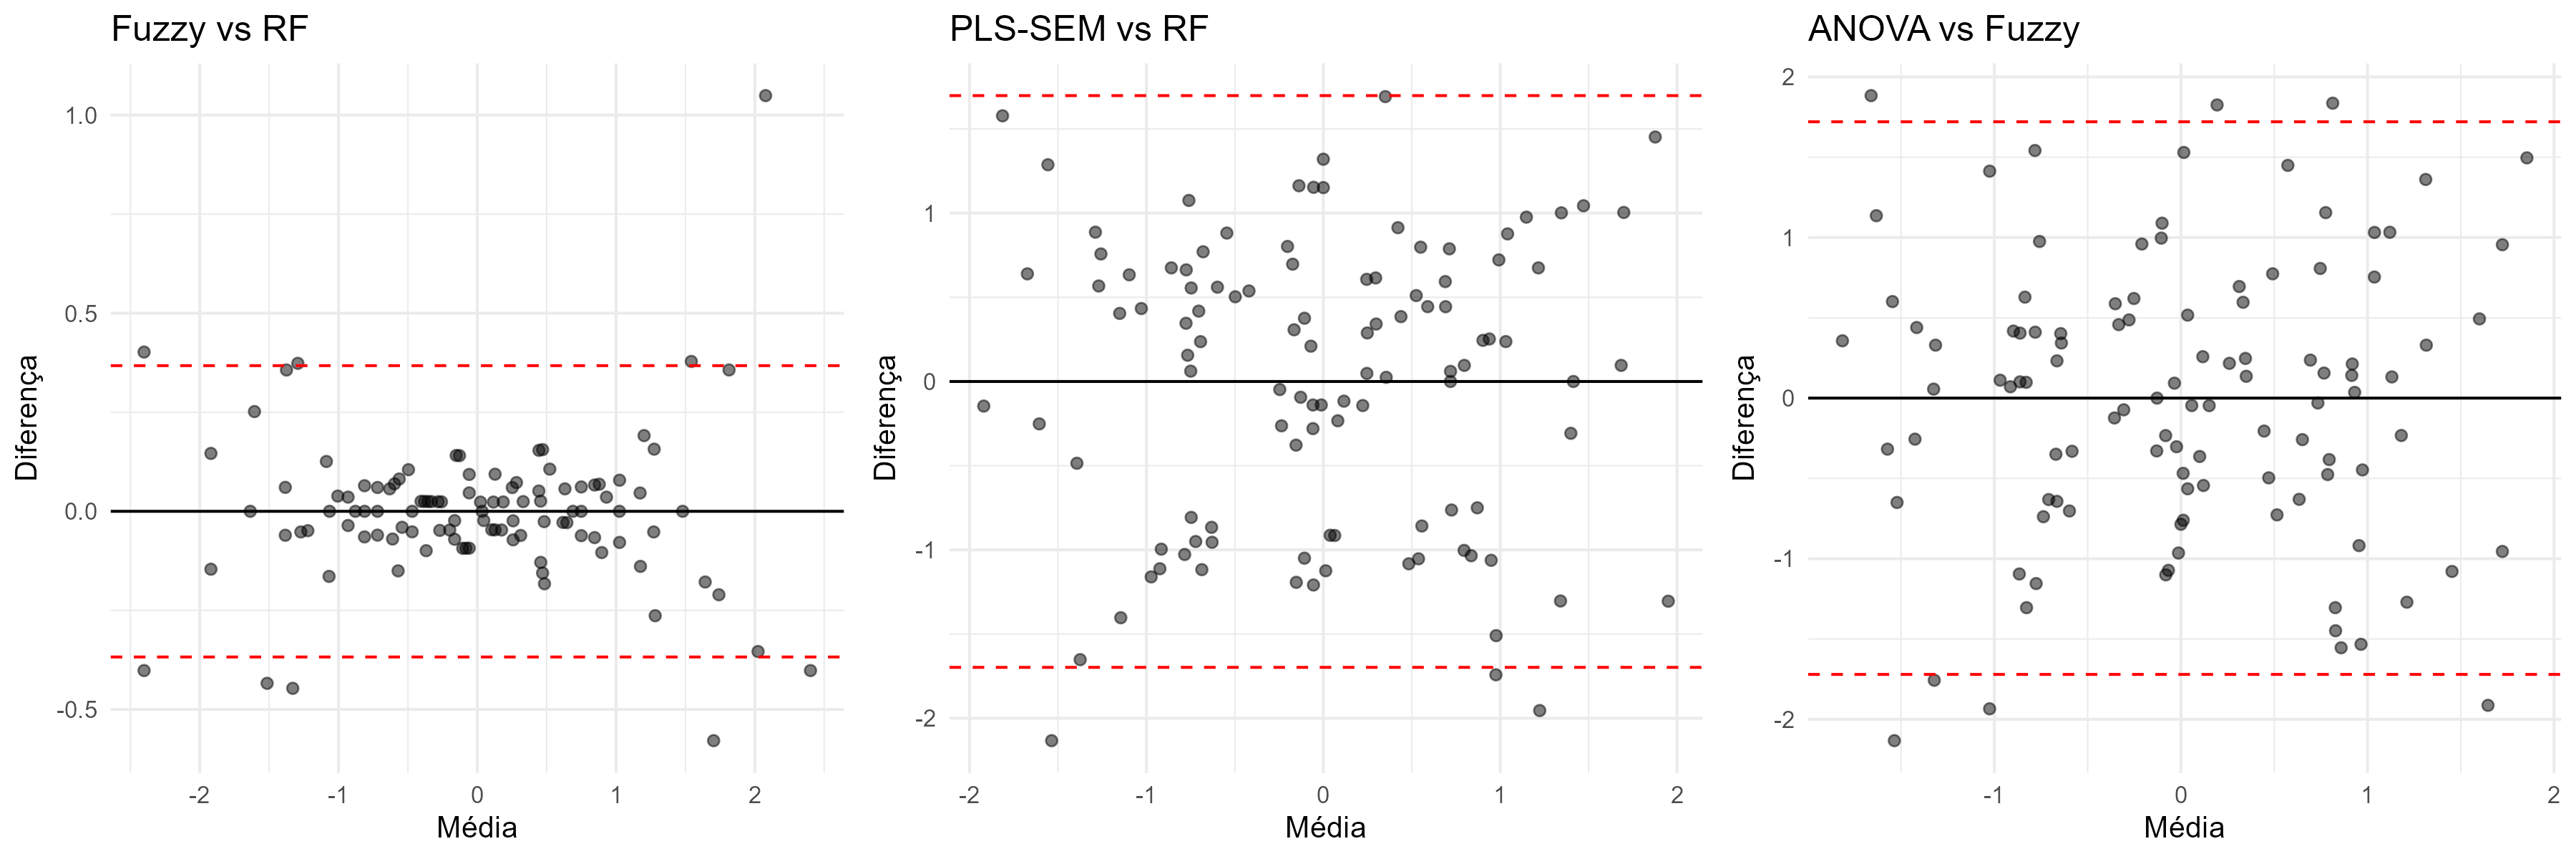
\includegraphics[width=\textwidth]{../../2-DADOS/3-FIGURAS/fig_blandaltman_panel.png}
\caption{Bland--Altman plots for three representative paradigm pairs (Blom scale).}\label{fig:ba_panel}
\smallskip\noindent\textit{Note:} Solid line, mean difference ($\bar{d} \approx 0$); dashed lines, limits of agreement at $\pm 1.96\,s_d$.
\end{figure}

Fuzzy ($\rho^2 = 0.990$) and MARS ($\rho^2 = 0.986$) align nearly perfectly with the identity diagonal in the 1:1 scatter plots (Fig.~\ref{fig:scatter1to1}), whereas ANOVA ($\rho^2 = 0.466$) and PLS-SEM ($\rho^2 = 0.446$) exhibit pronounced dispersion, with individual observations deviating by up to 1.5 Blom units from the 1:1 line \citep{Venkateswarlu2025}.

\begin{figure}[ht]
\centering
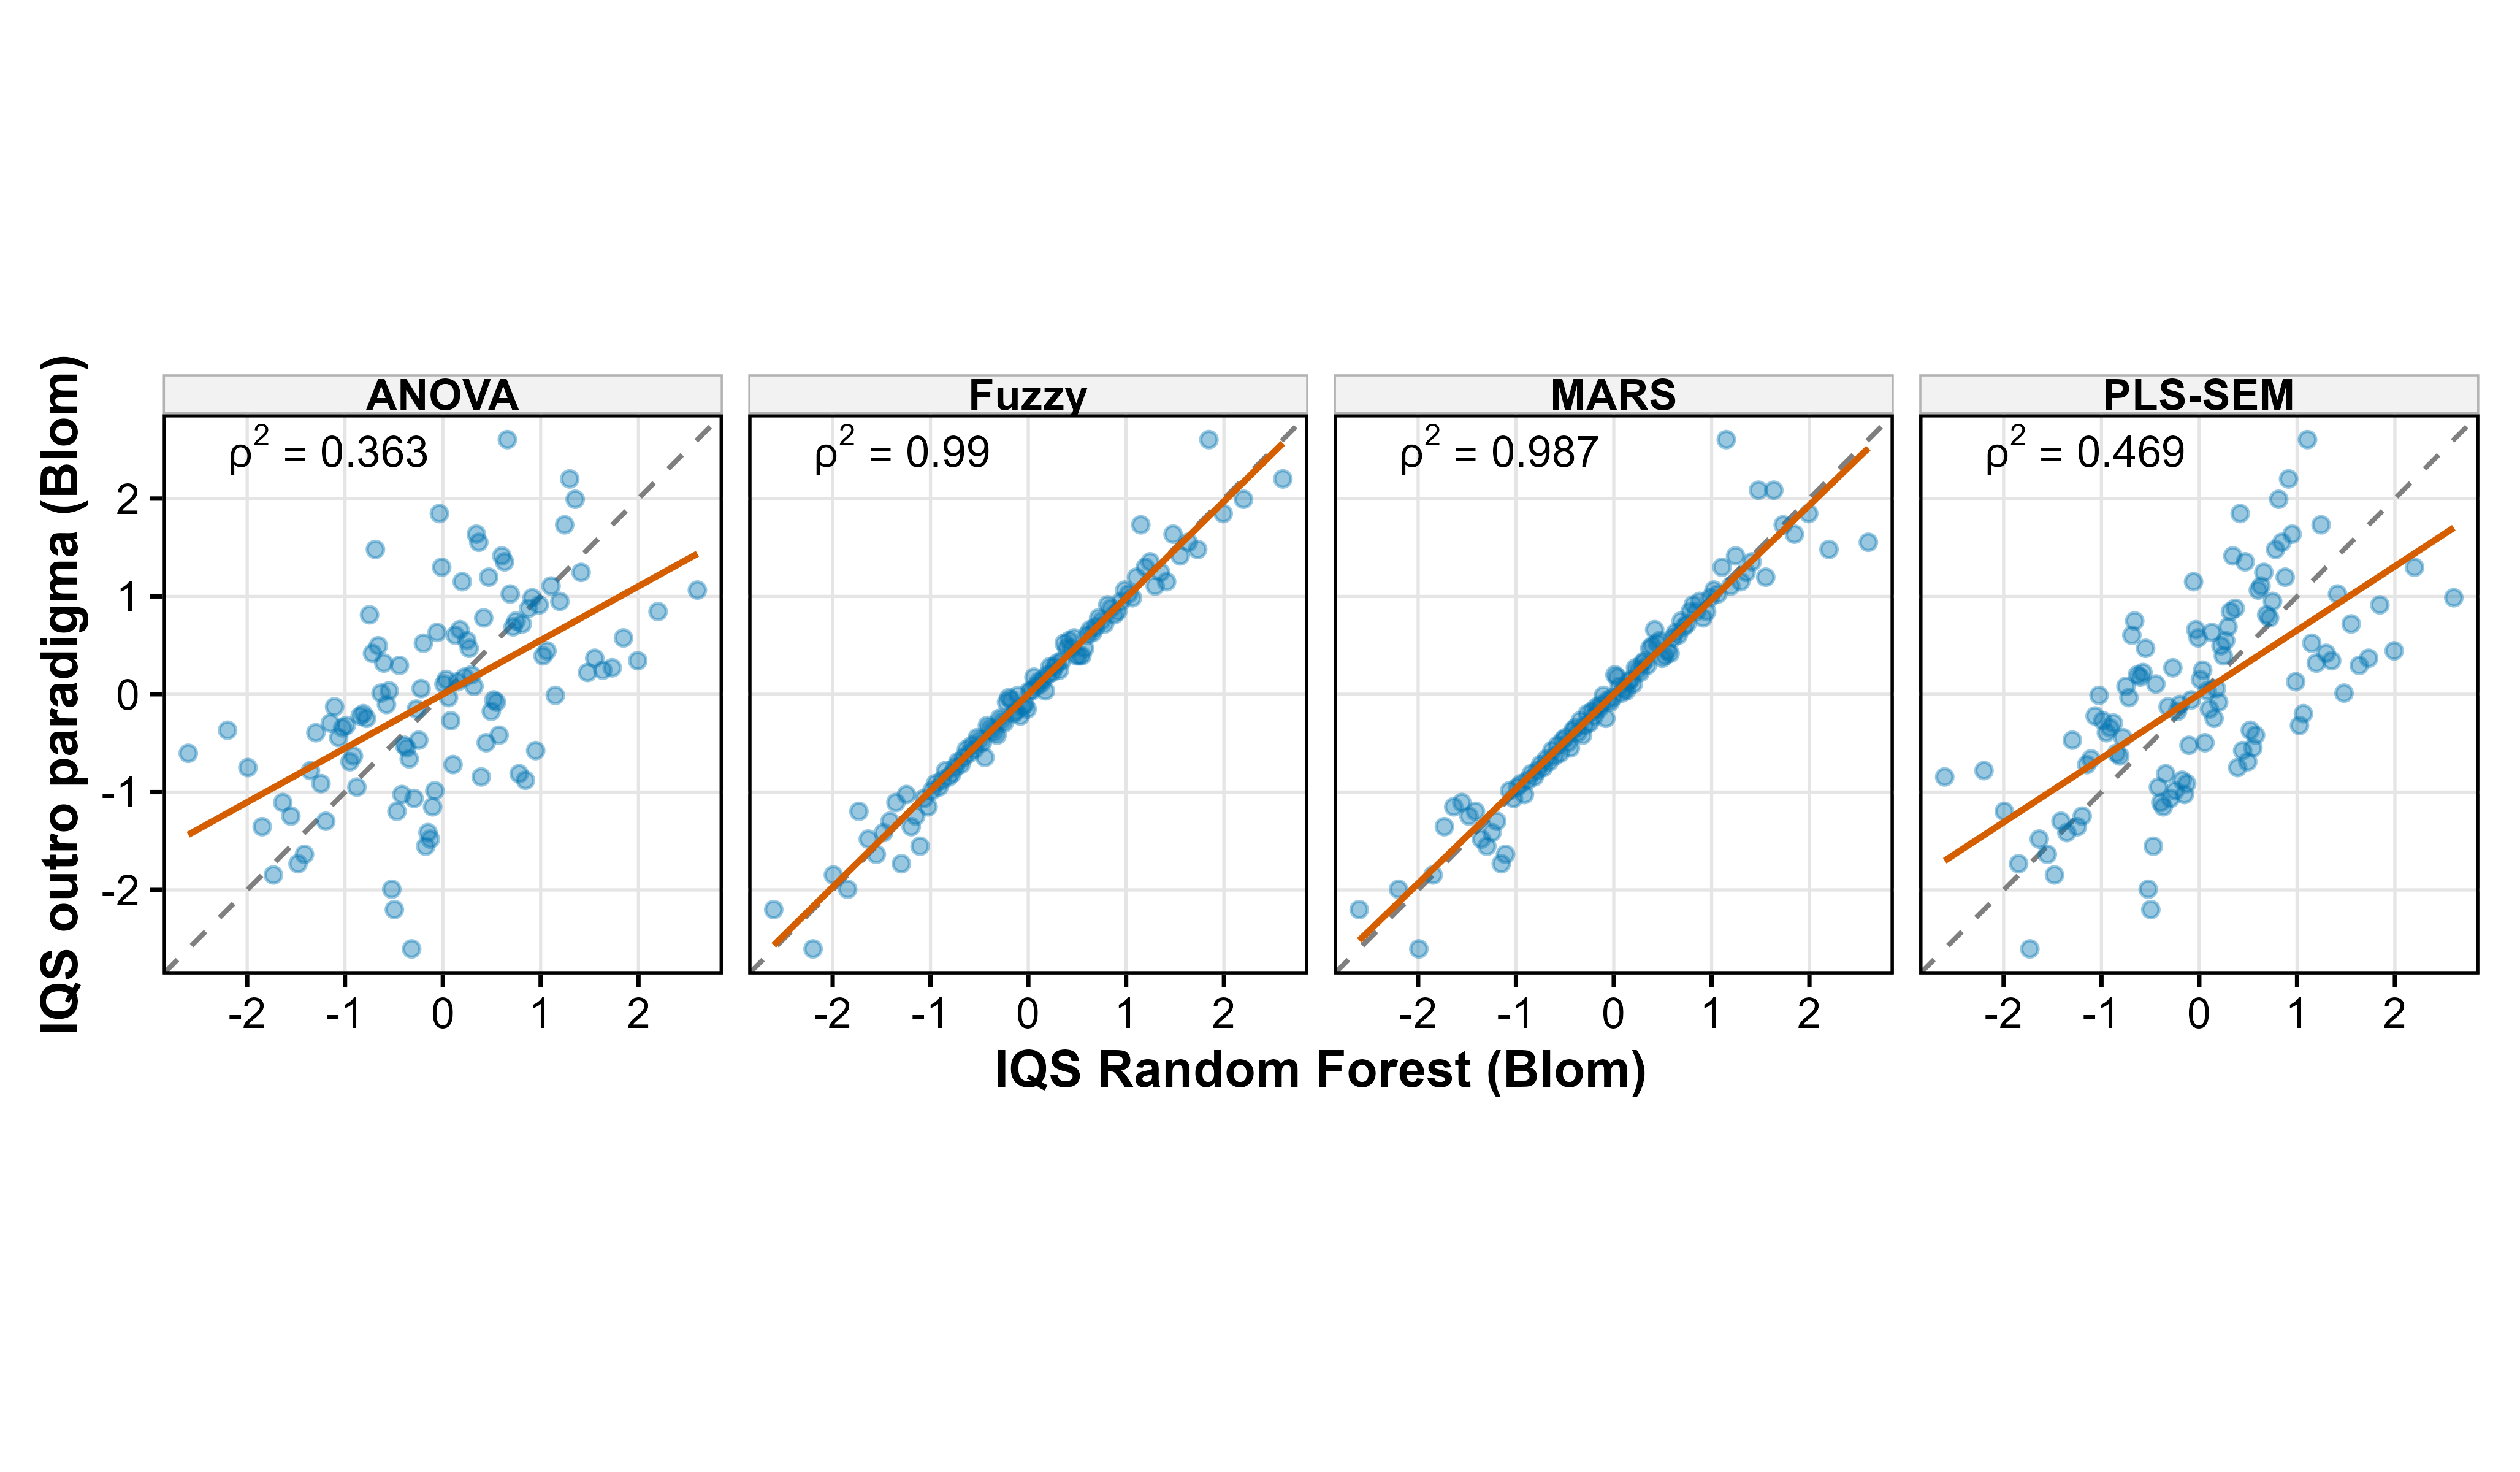
\includegraphics[width=\textwidth]{../../2-DADOS/3-FIGURAS/fig_scatter_1to1.png}
\caption{1:1 scatter plots of SQI (Blom scale) between each paradigm and RF as reference.}\label{fig:scatter1to1}
\smallskip\noindent\textit{Note:} Dashed line, identity; solid line, local regression. $\rho^2$ values annotated in each panel.
\end{figure}

This magnitude of deviation implies that, for a given observation, the diagnosis of ``high'' or ``low'' quality may be contingent on the paradigm when the conventional median threshold is adopted, a pattern that reinforces the need for concordance metrics in SQI assessment \citep{Liu2025}. \cite{Kahsay2025}, comparing eight SQI models (TDS/MDS $\times$ linear/nonlinear score $\times$ IQI/NQI) on degraded lands in Ethiopia, found that the nonlinear scoring function systematically produced indices 12--18\% higher than the linear score, with divergence amplified in low-quality soils, a pattern consistent with the fan-shaped bias observed in this study (Fig.~\ref{fig:ba_panel}). \cite{Zhang2024LDD}, in a wheat--maize rotation under conventional and conservation tillage in northern China, reported that the nonlinear-scored SQI detected conservation management benefits that the linear score did not distinguish, reinforcing the hypothesis that the analytical family, and not merely the indicator set, conditions index sensitivity.

The convergence among FIS, MARS, and RF is consistent with the hypothesis that these paradigms access the same variability subspace, defined by nonlinear relationships and high-order interactions among indicators that the linear model compresses or ignores \citep{Zeraatpisheh2020,Wadoux2020}. \cite{DosSantos2021} observed an analogous pattern in a Red Latosol under integrated production systems, with the fuzzy SQI detecting management differences that the classical additive protocol did not distinguish, supporting the generality of nonlinear convergence in tropical soils. The inclusion of the three chemical indicators attenuated the differentiation among analytical families, raising $\bar{\rho}_{\text{Lin-NL}}$ from 0.64 to 0.71 and rendering $H_2$ nonsignificant ($p = 0.38$). This suggests that chemical fertility provides between-plot variance information sufficiently linear to be captured by both PCA and nonlinear algorithms, partially homogenizing the rankings \citep{Rezaee2020}.

The amplitude of this disagreement varies with soil type and indexation approach. Divergences of up to 30\% between weighted additive and cumulative indices have been reported in soils with heterogeneous indicator distributions in central Iran \citep{Emami2024}, a magnitude consistent with the LoA of $\pm 1.25$ to $\pm 1.77$ observed in this study for pairs involving ANOVA. In saline coastal soils of India, concordance among three methods (SQI$_w$ additive, SQI$_n$ Nemoro, and SQI$_c$ cumulative) varied with salinity severity, being higher in intermediate-quality soils and lower at the extremes \citep{Mahajan2021}, a pattern resembling the heteroscedasticity documented in the Bland--Altman diagrams of this study.

PLS-SEM, by specifying linear paths among latent constructs but incorporating formative indicators (Mode~B) that partially capture nonlinearity in composition \citep{Diamantopoulos2008}, converged with ANOVA ($\rho = 0.83$) more than with the nonlinear block ($\rho \approx 0.66$), with LoA of $\pm 1.70$ that are of the same magnitude as the between-plot variability reported by \cite{Oliveira2020} for Acrisols under long-term no-tillage in northeastern Brazil. The divergence of ANOVA is consistent with the dependence on PCA-derived weights and linear combination of orthogonal scores, which lose information about higher-order interactions \citep{Andrews2002,Bünemann2018}, indicating that paradigm substitutability depends on the analytical family, not on the specific algorithm.

Previous comparisons among SQI methods had suggested that extreme ordering tends to be preserved even when absolute scores diverge by up to 15\% \citep{Mukherjee2014}, yet these comparisons remained restricted to variants of the same algorithmic family \citep{Chaudhry2024} or lacked a formal inter-rater concordance protocol \citep{Pacci2026}. The simultaneous confrontation of five families with structurally distinct assumptions, coupled with concordance metrics ($W$, ICC, Bland--Altman), enabled quantification of substitutability thresholds ($\rho > 0.99$ and LoA\,$< \pm 0.43$ for the FIS-MARS-RF block) that may serve as reference in future SQI benchmarking exercises \citep{Cherubin2016}.

The ordinal aggregation by Borda count, recognized as a strategy for consolidating divergent rankings in composite indicators \citep{Munda2012}, generated a meta-SQI with Spearman correlation $\geq 0.95$ relative to the FIS, MARS, and RF paradigms, a level consistent with functional interchangeability according to inter-rater concordance criteria \citep{Gwet2014}, whereas concordance with PLS-SEM ($\rho = 0.83$) and ANOVA ($\rho = 0.84$) remained in the moderate range.

The interpretation of the LoA followed the criterion of \cite{BlandAltman1999}, according to which two methods may be considered interchangeable when the limits of agreement are agronomically irrelevant. Pairs with $\rho > 0.99$ and LoA\,$< \pm 0.43$ satisfy this criterion for management ranking, whereas pairs with $\rho \approx 0.66$ and LoA\,$\approx \pm 1.70$ may produce divergences at intermediate positions without altering extremes. Pairs with $\rho \approx 0.83$ (ANOVA--PLS, LoA\,$\approx \pm 1.25$) represent moderate concordance that may be sufficient when the priority is historical comparability or causal interpretation.

The magnitude of the LoA between linear and nonlinear families ($\approx \pm 1.70$ on the Blom scale) implies operational risk for management recommendations based on intermediate ranking positions. Of the 12 tillage--cover crop combinations evaluated, six (50\%) switched classification tier (upper third $\leftrightarrow$ intermediate third) when the paradigm was changed from ANOVA to RF, which may alter practice prioritization in agricultural extension contexts.

The cost of an erroneous recommendation can be estimated by the yield differential between adjacent combinations in the ranking. Adopting CT-Cowpea (position 4 by RF, position 8 by ANOVA) instead of MT-Sunn hemp (stable at 2nd--4th position) may represent a yield loss on the order of 15--20\% in green corn production \citep{SantosJA2024}, equivalent to approximately 1,200--1,800\,kg\,ha$^{-1}$ of marketable ears in the Coastal Tablelands context. This magnitude suggests that paradigm choice is not economically neutral and may justify the inclusion of inter-paradigm sensitivity analysis in SQI assessments intended to inform soil conservation policies.

\subsection{Ranking by tillage--cover crop combination}\label{subsec:ranking}

The SQI score distribution by tillage--cover crop combination (Fig.~\ref{fig:boxplot_combo}) shows that minimum tillage with pigeon pea (MT-Pigeon pea) concentrated the highest median values across all five paradigms, with narrow interquartile ranges suggesting low internal variability for this combination. Conversely, conventional tillage with pigeon pea (CT-Pigeon pea) exhibited the lowest scores across all paradigms, with medians near 1.0 on the original scale. The comparatively superior performance of minimum tillage with pigeon pea, previously reported by \cite{Assuncao2023} for the 17th year of this same experiment, suggests temporal persistence of the management effect over at least five additional growing seasons, a result that may reflect the interaction between biological nitrogen fixation by pigeon pea and the magnitude of mechanical disturbance applied.

\begin{figure}[ht]
\centering
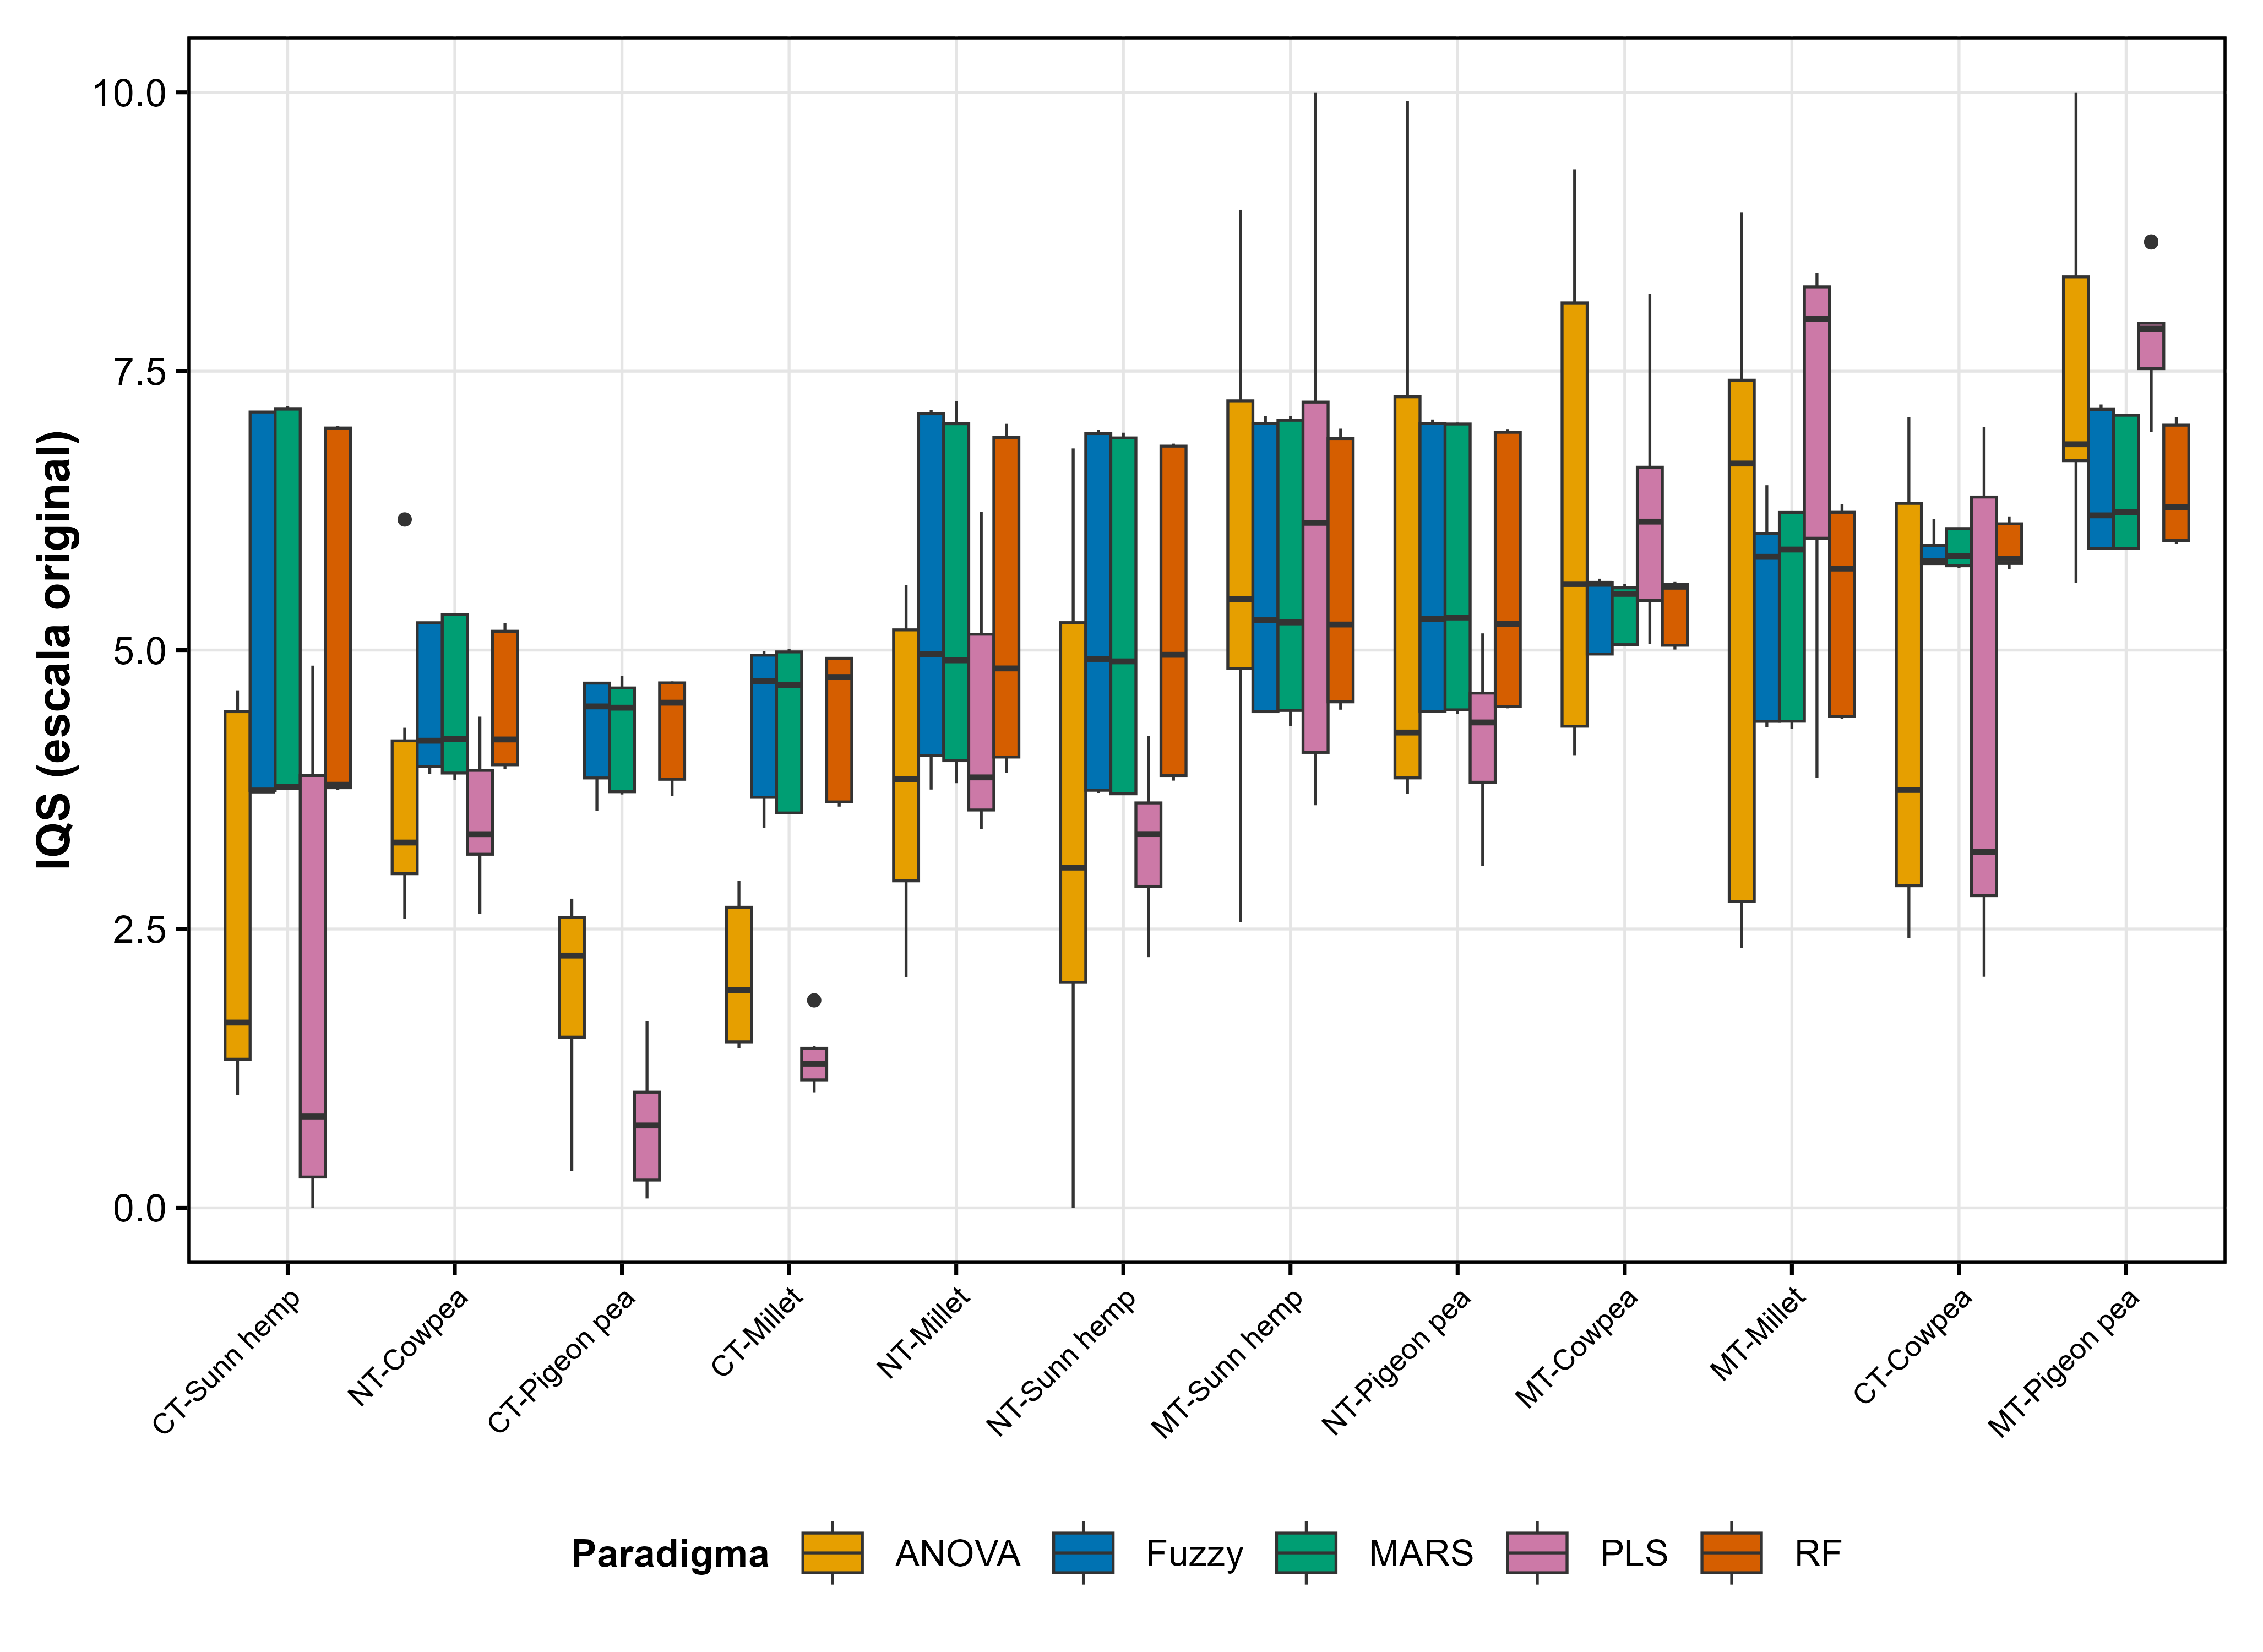
\includegraphics[width=\textwidth]{../../2-DADOS/3-FIGURAS/fig_boxplot_combo.png}
\caption{SQI distribution (original scale, 0--10) by tillage--cover crop combination and analytical paradigm.}\label{fig:boxplot_combo}
\smallskip\noindent\textit{Note:} Combinations ordered by Borda meta-SQI mean.
\end{figure}

Assessing green corn production in the same long-term plots in northeastern Brazil, \cite{SantosJA2024} observed that minimum tillage associated with cover crops produced yields 28\% higher than conventional tillage, with pigeon pea contributing to partial disruption of the cohesive layer through its deep pivoting root system ($> 2$~m).

This mechanism is consistent with observations by \cite{daSilva2021}, who found in a Red Acrisol under no-tillage that the corn/sunn hemp succession promoted an aggregate stability index ($> 90$\%) higher than the corn/fallow succession, attributing the difference to glomalin and continuous input of particulate organic matter in the legume rhizosphere.

The positioning of conventional tillage with pigeon pea in the last position across all five paradigms (Borda\,=\,20.9) suggests an apparent paradox that the structural destruction mechanism may explain. Plowing to 25\,cm followed by harrowing disrupts fungal hyphal networks and continuous biopores (diameter $> 75$\,\textmu m) created by the pivoting root system of pigeon pea, negating the benefits of biological N$_2$ fixation (50--200\,kg\,N\,ha$^{-1}$\,yr$^{-1}$) and cohesive-layer disruption \citep{Peoples2009}.

This disconnect between N input and structural preservation explains why the same cover crop species simultaneously occupies the first (MT-Pigeon pea) and last (CT-Pigeon pea) ranking positions, since the agronomic benefit of the legume is contingent on the maintenance of soil physical integrity. \cite{Thomaz2022}, in a 23-year experiment with tobacco in southern Brazil, documented a 45\% reduction in the aggregate stability index and an erodibility increase ($K$-USLE from 0.018 to 0.031~Mg ha h ha$^{-1}$ MJ$^{-1}$ mm$^{-1}$) under conventional tillage compared to no-tillage, corroborating that repeated mechanical disturbance overrides the rhizospheric effect of the legume. Intermediate positions, however, exhibited inversions among paradigms for 50\% of the tillage--cover crop combinations (6 of 12). CT-Cowpea occupied 2nd position by Fuzzy, MARS, and RF, but 8th by ANOVA, illustrating the largest inversion observed. MT-Sunn hemp rose to 2nd position in PLS-SEM but was placed 4th by Fuzzy and MARS.

This inversion is consistent with the differential sensitivity of paradigms to the relative contribution of physical versus yield indicators, since the ANOVA MDS protocol applies PCA-derived weights that equalize domains, whereas the nonlinear paradigms weight by algorithm-estimated predictive capacity \citep{Chaudhry2024}. \cite{Fernandes2022}, studying aggregation under no-tillage with different successions (corn/sunn hemp vs.\ corn/pearl millet vs.\ fallow), found that the legume succession promoted higher particulate organic carbon content and aggregate stability index in the 0--0.10~m layer, whereas the grass succession favored subsurface macroporosity (0.10--0.20~m). This depth- and domain-dependent differentiation may explain why paradigms that rank by global predictive capacity (RF, MARS, FIS) place CT-Cowpea above MT-Cowpea, while ANOVA, which equalizes weights among domains via PCA, inverts this order.

PLS-SEM also exhibited occasional divergences, placing NT-Pigeon pea in 5th position (vs.\ 2nd--3rd in the others), which may stem from the exclusion of four indicators due to multicollinearity in the structural model specification. \cite{OliveiraFCC2024}, assessing oxidizable fractions of soil organic carbon in an Acrisol under long-term conservation management in northeastern Brazil, observed that no-tillage with pigeon pea accumulated a higher proportion of labile carbon (F1 fraction) in the 0--0.05~m layer compared to other systems, which may sensitize nonlinear models that capture relationships between carbon fractions and yield that PLS-SEM, with lower dimensionality, does not retain. These findings indicate that, for management decisions based on intermediate ranking positions, paradigm choice may alter the final recommendation, reinforcing the utility of the Borda meta-SQI as a consensus metric \citep{Lin2010}. The consolidated ordinal quantification of these positions (Table~\ref{tab:ranking}) shows convergence at the extremes (MT-Pigeon pea = 93.7; CT-Pigeon pea = 20.9) and enables localization of each inversion discussed.

\begin{table}[ht]
\caption{Ranking of the 12 tillage--cover crop combinations by five paradigms and Borda meta-SQI.}\label{tab:ranking}
\begin{tabular*}{\textwidth}{@{\extracolsep\fill}llcccccc}
\toprule
Tillage & Cover crop & ANOVA & Fuzzy & PLS & MARS & RF & Borda \\
\midrule
MT & Pigeon pea & 1 & 1 & 1 & 1 & 1 & 93.7 \\
MT & Sunn hemp    & 3 & 4 & 2 & 4 & 3 & 70.0 \\
MT & Pearl millet       & 4 & 5 & 3 & 5 & 5 & 68.8 \\
CT & Cowpea         & 8 & 2 & 7 & 2 & 2 & 66.4 \\
MT & Cowpea         & 5 & 6 & 4 & 6 & 6 & 66.3 \\
NT & Pigeon pea & 2 & 3 & 5 & 3 & 4 & 65.9 \\
NT & Pearl millet       & 7 & 7 & 6 & 7 & 7 & 55.6 \\
NT & Sunn hemp    & 6 & 8 & 8 & 8 & 8 & 50.9 \\
CT & Sunn hemp    &10 & 9 &10 & 9 & 9 & 36.4 \\
NT & Cowpea         & 9 &10 & 9 &10 &10 & 34.6 \\
CT & Pearl millet       &11 &11 &11 &12 &11 & 24.4 \\
CT & Pigeon pea &12 &12 &12 &11 &12 & 20.9 \\
\botrule
\end{tabular*}
\smallskip\noindent\textit{Note:} NT, no-tillage; CT, conventional tillage; MT, minimum tillage. Higher Borda values indicate better integrated soil quality.
\end{table}

The convergence at the extremes of Table~\ref{tab:ranking} suggests that the superior performance of minimum tillage with pigeon pea (Borda\,=\,93.7) and the inferior performance of conventional tillage with pigeon pea (Borda\,=\,20.9) tend to be stable across paradigms and may be incorporated into agronomic recommendations with lower dependence on the analytical method. Sunn hemp under minimum tillage rose to the second position (Borda\,=\,70.0), reinforcing the synergistic effect of legumes with minimal soil disturbance. In contrast, recommendations involving combinations situated between the 2nd and 7th positions benefit from explicit indication of the paradigm used and, preferably, from inter-paradigm sensitivity analysis assessing rank stability. This practice of methodological transparency is particularly relevant in agricultural extension contexts and public policy formulation for soil conservation, where the recommendation of a management system may mobilize long-term investments whose consequences exceed conventional statistical uncertainty \citep{Majid2025}.

The results of this benchmarking suggest that smallholder farmers of the Coastal Tablelands may benefit from adopting minimum tillage with a single leveling harrow pass (maximum depth of 10\,cm), combined with a pigeon pea (15--20\,kg\,ha$^{-1}$) and pearl millet (5--8\,kg\,ha$^{-1}$) intercrop at a 75:25 seed-weight ratio, sown 60--90 days before corn. Maintaining at least 50\% residual cover on the surface until main-crop sowing and monitoring structural quality through VESS (Visual Evaluation of Soil Structure) every two cycles (alert threshold at SQ\,$\geq$\,2.5) complete the operational protocol derived from inter-paradigm convergence.

\subsection{Sample-size sensitivity}\label{subsec:sensitivity_disc}

Inter-paradigm concordance exhibited strong sample-size dependence in the stratified Monte Carlo simulations (Fig.~\ref{fig:mc_box}), with $\bar{W}$ increasing sharply from 0.542 ($s = 0.163$) at $n = 15$ to 0.809 ($s = 0.066$) at $n = 30$. The variation interval contracted simultaneously, with the standard deviation decreasing from 0.163 to 0.033 between $n = 15$ and $n = 100$, indicating that divergence among analytical families is governed predominantly by sample size.

\begin{figure}[ht]
\centering
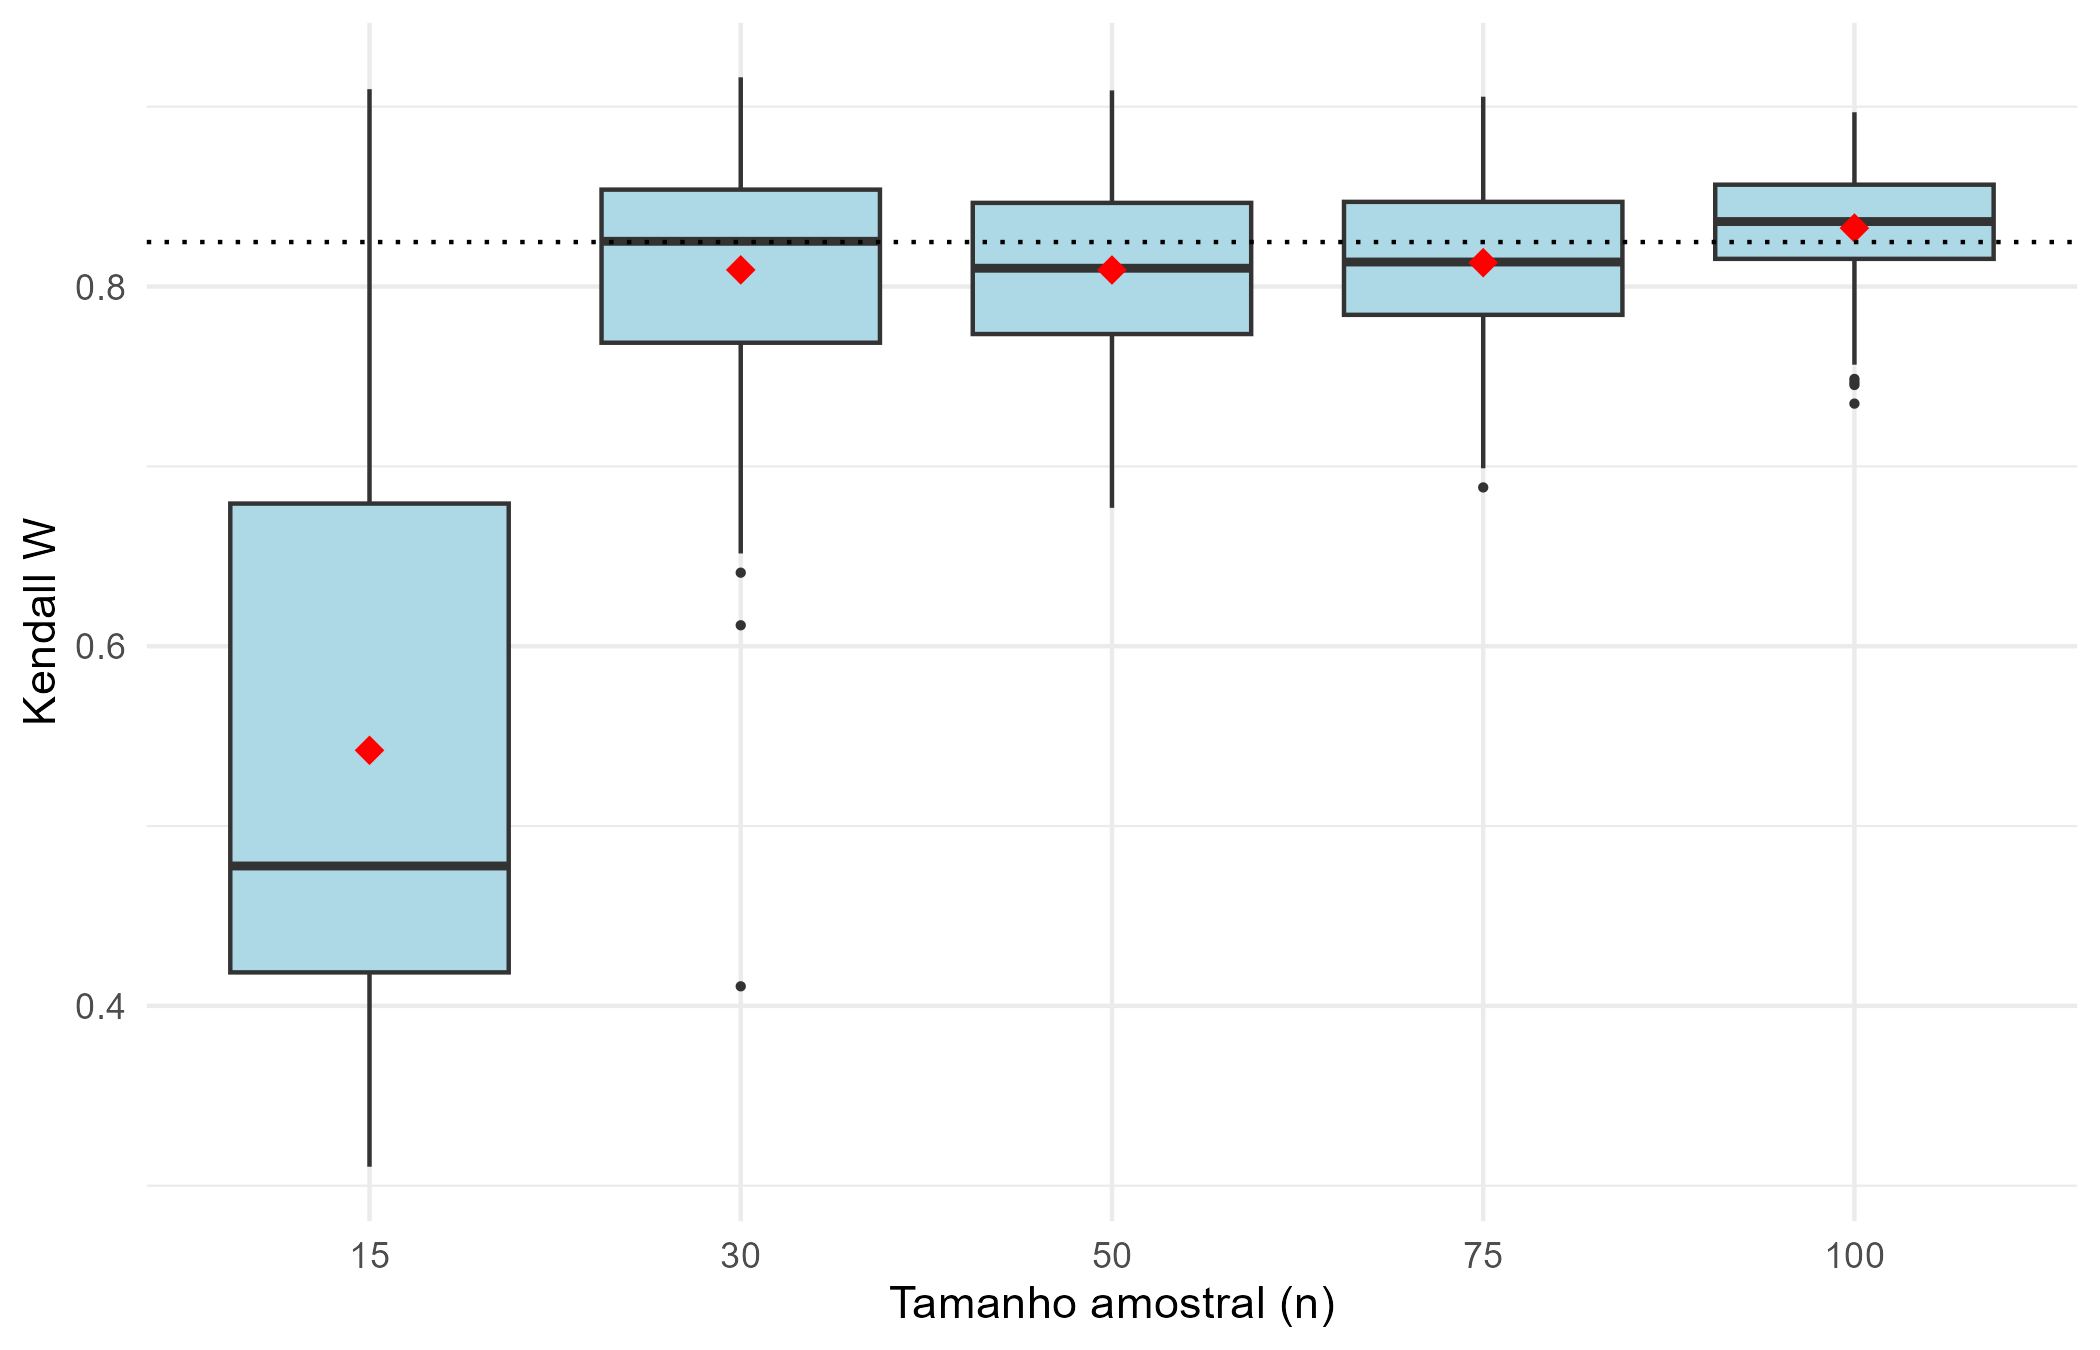
\includegraphics[width=0.75\textwidth]{../../2-DADOS/3-FIGURAS/fig_mc_sensitivity.png}
\caption{Distribution of Kendall's coefficient ($W$) as a function of sample size ($n$), obtained from 200 stratified Monte Carlo iterations by factorial design cell.}\label{fig:mc_box}
\smallskip\noindent\textit{Note:} Diamonds indicate the mean; dotted line indicates $W$ for the full sample ($n = 108$).
\end{figure}

From $n = 30$ onward, $\bar{W}$ stabilized within the 0.809--0.833 interval, signaling that the incorporation of chemical indicators reduced the concordance stabilization threshold from $n \approx 50$ (15-indicator model) to $n \approx 30$, below which algorithmic uncertainty supersedes real inter-paradigm variability. The GLS line fitted on $\log(n)$ indicated a positive trend ($\hat{\beta}_1 = 0.056$), although the effect did not reach conventional significance ($p = 0.235$), and the 2.5th--97.5th percentile band progressively converged toward the full-sample reference.

The lack of significance may reflect both the small number of sample-size levels ($k = 5$), which limits the statistical power of the test \citep{Mundform2005}, and the abrupt jump in $\bar{W}$ between $n = 15$ and $n = 30$ that violates the log-linear sample-size premise. \cite{Adak2023}, applying SQI under contrasting tillage, residue, and nitrogen management in a wheat--maize rotation on the Indo-Gangetic Plain, found that samples with $n < 30$ inflated the uncertainty of PCA-derived weights, destabilizing treatment rankings and producing position inversions among management practices that, with the full sample ($n = 96$), were statistically distinct. This pattern indicates that subsampling introduces variability that supersedes real differences among paradigms, generating disagreements not observed in the full sample. Benchmarking exercises conducted with $n < 30$ therefore operate in a zone of high instability ($\bar{W} < 0.54$, $s > 0.16$), where conclusions about the superiority or inferiority of a paradigm are indistinguishable from sampling noise, whereas $n \geq 30$ appears sufficient to isolate the algorithmic signal when the indicator vector includes the chemical domain.

\subsection{Implications for monitoring and transferability}\label{subsec:implications}

When the interest lies in ranking tillage--cover crop combinations in datasets with $n \geq 50$, any representative of the nonlinear block (FIS, MARS, or RF) may be adopted with low risk of inversion ($\rho > 0.99$), potentially dispensing with paradigm sensitivity analysis. If interpretability of causal paths among soil domains is a priority, as recommended in composite indicator assessments \citep{Cardoso2013}, PLS-SEM offers an alternative with moderate uncertainty relative to the nonlinear block (LoA\,$\approx \pm 1.72$), although the exclusion of indicators due to multicollinearity may compromise physical domain representativeness. The ANOVA/MDS paradigm remains useful for compatibility with the extensive body of studies that adopted the \cite{Andrews2002} protocol and for datasets with a small number of indicators ($q < 10$), a condition under which the predictive precision gain of nonlinear methods tends to be marginal \citep{Bünemann2018}. This selection protocol, schematized in Fig.~\ref{fig:flowchart}, may serve as a reference for researchers and extension agents who need to justify the methodological choice and quantify the associated uncertainty in soil quality assessments.

\begin{figure}[!htb]
\centering
\resizebox{\textwidth}{!}{%
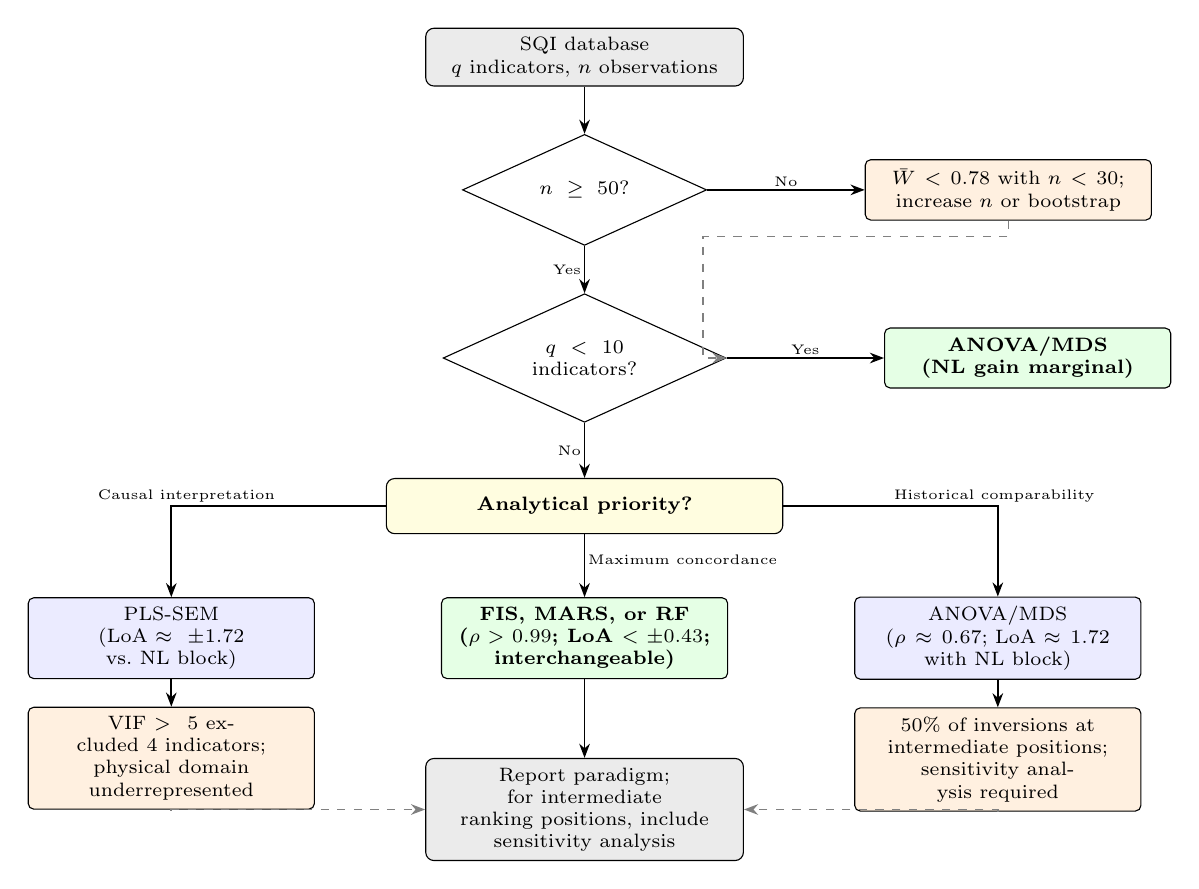
\begin{tikzpicture}[
    % --- node styles ---
    startend/.style={rectangle, rounded corners=3pt, minimum width=4cm,
        minimum height=0.6cm, text centered, draw=black, fill=black!8,
        font=\scriptsize, text width=3.8cm},
    dec/.style={diamond, aspect=2.2, minimum width=0.8cm,
        text centered, draw=black, fill=white,
        font=\scriptsize, text width=2.4cm, inner sep=1pt},
    prio/.style={rectangle, rounded corners=3pt, minimum width=5cm,
        minimum height=0.7cm, text centered, draw=black, fill=yellow!12,
        font=\scriptsize\bfseries, text width=4.8cm},
    rec/.style={rectangle, rounded corners=2pt, minimum width=3.6cm,
        minimum height=0.5cm, text centered, draw=black, fill=green!10,
        font=\scriptsize\bfseries, text width=3.4cm},
    proc/.style={rectangle, rounded corners=2pt, minimum width=3.6cm,
        minimum height=0.5cm, text centered, draw=black, fill=blue!8,
        font=\scriptsize, text width=3.4cm},
    warn/.style={rectangle, rounded corners=2pt, minimum width=3.6cm,
        minimum height=0.5cm, text centered, draw=black, fill=orange!12,
        font=\scriptsize, text width=3.4cm},
    % --- arrow / label styles ---
    arr/.style={-{Stealth[length=1.8mm]}, semithick},
    lbl/.style={font=\tiny, fill=white, inner sep=1pt},
    node distance=0.55cm and 1.6cm
]

%%% ================= ROW 0: INPUT =================
\node (start) [startend]
    {SQI database\\$q$ indicators, $n$ observations};

%%% ================= ROW 1: SAMPLE GATE =================
\node (d1) [dec, below=0.6cm of start] {$n \geq 50$?};
\node (w1) [warn, right=2cm of d1]
    {$\bar{W} < 0.78$ with $n < 30$;\\increase $n$ or bootstrap};

%%% ================= ROW 2: DIMENSIONALITY GATE =================
\node (d2) [dec, below=0.6cm of d1] {$q < 10$\\indicators?};
\node (r_lowq) [rec, right=2cm of d2]
    {ANOVA/MDS\\(NL gain marginal)};

%%% ================= ROW 3: PRIORITY BRANCH =================
\node (prio) [prio, below=0.7cm of d2]
    {Analytical priority?};

%%% ================= ROW 4: THREE RECOMMENDATIONS =================
\node (nlrec) [rec, below=0.8cm of prio]
    {FIS, MARS, or RF\\($\rho > 0.99$; LoA $< \pm 0.43$;\\interchangeable)};
\node (pls)   [proc, left=1.6cm of nlrec]
    {PLS-SEM\\(LoA $\approx \pm 1.72$\\vs.\ NL block)};
\node (anova) [proc, right=1.6cm of nlrec]
    {ANOVA/MDS\\($\rho \approx 0.67$; LoA $\approx 1.72$\\with NL block)};

%%% ================= ROW 5: CAVEATS =================
\node (pls_w)   [warn, below=0.35cm of pls]
    {VIF $> 5$ excluded 4 indicators;\\physical domain underrepresented};
\node (anova_w) [warn, below=0.35cm of anova]
    {50\% of inversions at\\intermediate positions;\\sensitivity analysis required};

%%% ================= ROW 6: OUTPUT =================
\node (endnode) [startend, below=1cm of nlrec]
    {Report paradigm; for intermediate\\ranking positions, include\\sensitivity analysis};

%%% ================= ARROWS =================
%% Binary gates
\draw [arr] (start) -- (d1);
\draw [arr] (d1) -- node[lbl, left] {Yes} (d2);
\draw [arr] (d1) -- node[lbl, above] {No} (w1);
\draw [arr] (d2) -- node[lbl, left] {No} (prio);
\draw [arr] (d2) -- node[lbl, above] {Yes} (r_lowq);

%% Triple branch from PRIORITY
\draw [arr] (prio.south) -- node[lbl, right, pos=0.4]
    {Maximum concordance} (nlrec);
\draw [arr] (prio.west) -| node[lbl, above left, pos=0.25]
    {Causal interpretation} (pls);
\draw [arr] (prio.east) -| node[lbl, above right, pos=0.25]
    {Historical comparability} (anova);

%% Caveats
\draw [arr] (pls) -- (pls_w);
\draw [arr] (anova) -- (anova_w);

%% Convergence to output
\draw [arr] (nlrec) -- (endnode);
\draw [arr, dashed, gray] (pls_w.south) |- (endnode.west);
\draw [arr, dashed, gray] (anova_w.south) |- (endnode.east);

%% Return: $n < 50$
\draw [arr, dashed, gray] (w1.south) |- ([yshift=-0.2cm]w1.south) -| ([xshift=1.5cm]d1.south) |- (d2.east);

\end{tikzpicture}%
}% end resizebox
\caption{Decision flowchart for SQI paradigm selection.}\label{fig:flowchart}
\smallskip\noindent\textit{Note:} Green boxes, primary recommendation; blue boxes, alternative with caveat; orange boxes, operational warning; yellow box, multi-criteria branching node. $\rho$ and LoA thresholds derived from Table~\ref{tab:blandaltman}; rank inversions documented in Table~\ref{tab:ranking}.
\end{figure}

The generalization of these findings requires caution. The data originate from an experiment conducted on an Acrisol with a cohesive layer \citep{LimaNeto2010} under an As$'$ climate, a condition under which nonlinear relationships among indicators may be accentuated by the subsurface physical impediment. Soils without physical restriction, or systems with lower practice diversity, could exhibit higher inter-paradigm concordance, reducing differentiation among analytical families. \cite{Zhao2022}, in a Mollisol subjected to 19 years of conservation management in China, found that physical attributes (aggregate stability, porosity) were more sensitive to tillage type than chemical indicators, which responded predominantly to fertilization.

In tropical soils with a cohesive layer, the contribution of physical attributes to SQI tends to be compressed by low spatial differentiation at the sampled depth, which may amplify divergence among paradigms competing for explainable variance in few physical indicators. Comparisons with Ultisols from Southeast Asia reinforce the regional applicability of the findings: \cite{Pheap2025}, in a rice--legume rotation experiment in Cambodia, found that fuzzy inference detected conservation management benefits that the additive SQI did not distinguish, with concordance among nonlinear paradigms ($\rho > 0.96$) similar to that observed in this study. \cite{Briliawan2022}, in an agroforestry system on an Indonesian Ultisol, reported convergence between RF and FIS (LoA\,$\approx \pm 0.51$), corroborating that nonlinear block substitutability may be generalized to tropical soils of low intrinsic fertility. Application of this same framework to datasets from other soil classes, particularly clayey Oxisols of the Cerrado, where \cite{DosSantos2021} indicated that the fuzzy SQI differentiated among cover systems, constitutes a promising direction for consolidating the concordance thresholds proposed here.


%% ================================================================
%%                    SECTION 5: CONCLUSION
%% ================================================================
\section{Conclusion}\label{sec:conclusion}

The five paradigms converged in identifying extreme managements, yet 50\% of intermediate combinations shifted position by analytical family, indicating that aggregation method choice may condition conservation recommendations. Nonlinear paradigms (FIS, MARS, RF) were practically interchangeable, whereas methods based on linear compression tended to diverge from the nonlinear block, suggesting that exclusive adoption of linear approaches may introduce additional uncertainty into the multivariate assessment of management systems. Chemical-domain indicator inclusion reduced the sample-size threshold for stabilizing inter-paradigm concordance, and minimum tillage with legumes (pigeon pea) appears the most consistent combination across the approaches tested. SQI assessments intended to inform conservation policies may benefit from including at least one nonlinear paradigm and inter-paradigm sensitivity analysis for intermediate ranking positions.

\backmatter


\bmhead{Acknowledgments}

The authors thank the technicians of the Campus Rural of the Universidade Federal de Sergipe for support in conducting the long-term experiment and collecting soil samples.

\section*{Declarations}

\begin{itemize}
\item \textbf{Funding:}

This study was financed in part by the Coordena\c{c}\~{a}o de Aperfei\c{c}oamento de Pessoal de N\'{i}vel Superior -- Brazil (CAPES) -- Finance Code 001 and by the Conselho Nacional de Desenvolvimento Cient\'{i}fico e Tecnol\'{o}gico (CNPq).
\item \textbf{Conflict of interest:}

The authors declare no competing interests.
\item \textbf{Ethics approval:}

Not applicable.
\item \textbf{Consent for publication:}

Not applicable.
\item \textbf{Data and code availability:}

The anonymized dataset and all analysis routines (R and Python) used in this study are available at [REPOSITORY URL]. Supplementary Tables S1--S4 present the complete ANOVA output, fuzzy rule base, PLS-SEM path coefficients, and variable importance rankings.
\item \textbf{Author contributions:}

\textbf{A. Pedrotti}: Supervision, Project administration, Resources, Investigation, Funding acquisition. \textbf{L.D.V. Santos}: Conceptualization, Methodology, Software, Formal analysis, Visualization, Writing -- original draft. \textbf{J.A. Santos}: Investigation, Data curation. \textbf{J.S. Ara\'{u}jo}: Investigation, Data curation. \textbf{R.N. Ara\'{u}jo Filho}: Methodology, Validation, Writing -- review \& editing. \textbf{E.G. Silva}: Investigation, Data curation. \textbf{B.M.S. Andrade}: Investigation, Data curation. \textbf{F.S.R. Holanda}: Supervision, Resources, Funding acquisition. All authors read and approved the final manuscript.
\end{itemize}

\begin{appendices}

\section{Complete fuzzy rule base}\label{secA2}

%% [TO BE INSERTED]

\section{PLS-SEM path coefficients and diagnostics}\label{secA3}

%% [TO BE INSERTED]

\end{appendices}

\bibliography{sn-bibliography}% common bib file

\end{document}
